\thesischapterexordium

\section{研究工作的背景与意义}

视觉问答是近几年学界新兴研究的热门方向之一。得益于神经网络架构在自然语言处理和图像识别相关任务的成功应用,学界将研究的视线移向对系统智能要求更高的视觉问答任务。视觉问答任务是一类输入为图像和用自然语言表达的文本问题,输出为基于图像内容理解并且用自然语言方式呈现的答案的计算机视觉任务。简而言之,任务目标是构建一个像人类智能一样的问答系统——能够从给定的图片中,抽象凝结出图中物体的类别、空间关系、活动、场景等高阶信息;并根据问题的不同,针对性得给出合理的答案。

视觉问答的问题类型包含二值的是否问题\citing{krishna2017visual,zhu2016visual7w,andreas2015deep}、多选问题\citing{antol2015vqa,zhu2016visual7w}、开放性问题\citing{antol2015vqa},涉及诸多计算机视觉中的子任务\citing{kafle2017visual},例如:
\begin{description}[labelindent=2em, leftmargin=6em, style=sameline]
\item [物体识别]——图片中有哪些动物?
\item [物体检测]——图片中是否有小狗?
\item [属性分类]——图片中小狗的眼睛是什么颜色?
\item [场景分类]——图片中的小狗在什么地方?
\item [计数问题]——图片中有几只小狗?
\end{description}
除了以上列出的集中问题类型以外,在真实的人类交流中,更多的是具有更深层次、更复杂的问题。例如:“图片中有什么东西在伞下?”——需要能准确识别物体的空间位置关系、“图片中的交通路口是否可以通行?”——需要基于常识的推理、“图片中的汽车属于什么品牌?”——需要基于外部专业知识库提供隐藏信息。

对问题中涉及的计算机视觉任务细分,我们可以将视觉问答分为识别和推理两大任务范畴。就识别任务而言,包括物体识别、物体检测、属性分类、计数问题、空间关系判定,此类任务在以往的计算机视觉的研究中已经达到了较高的识别准确率,在某些物体识别和物体检测任务上已经能迫近甚至超越人类水平,虽然识别任务中仍然有许多值得研究的部分,但从研究的结构和难度上来看,只能算是相对简单的“点问题”。与之对应的便是更为复杂的”逻辑推演问题“,包括场景分类、知识库推理,常识推理可以被视为一种“隐知识库推理”。识别任务是逻辑推演的“前奏”,准确的识别将构成逻辑推演的“节点”,而逻辑链条中节点之间的“有向线段”则代表推理的过程(如图\ref{logic}),推理过程的构建才是推理任务的复杂之处,也是视觉问答任务的“最璀璨的明珠”。
\begin{figure}[H]
	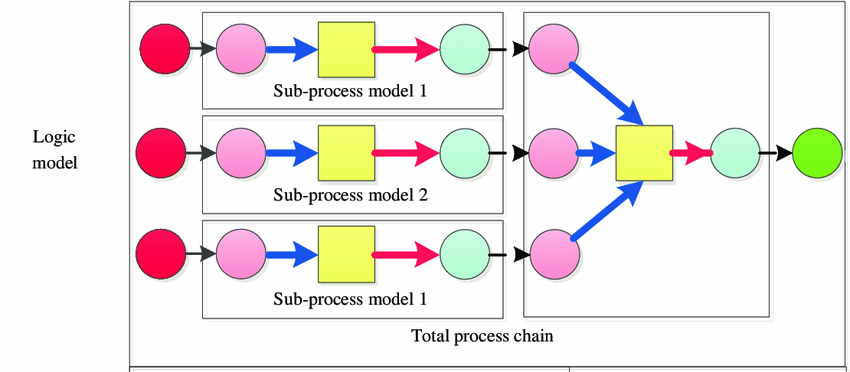
\includegraphics[width=0.8\textwidth]{logic.png}
	\caption{逻辑链中的“节点”是文本或图像上的关键信息,例如物体名称、类别、属性、关系等,“有向线段”表示“节点”间的逻辑关系}
	\label{logic}
\end{figure}

视觉问答主要涉及计算机视觉、自然语言处理、知识表达与推理三个领域。作为一个多学科交叉的领域,想实现高准确率的系统表现,既依托单个分支下理论、算法、应用系统的快速发展,作为其基础设施;同时还对各算法、子系统结合时的性能融合、体系结构提出了更多、更新的研究要求。这既是多学科高度融合状况下的挑战,也是令人兴奋不已的。正是由于视觉问答任务需要处理语言和图像两种重要的数据类型,这使得智能体更像人类一般思考和推理。智能体的“视觉系统”能够接收含有深层次信息的图像源;智能体的“神经系统”能解析图像信息和理解语言内涵;智能体的“语言系统”能够遣词造句,输出人类可理解的语言形式。因此视觉问答被认为是人类构建“人工智能完全体”的重要一步\citing{ antol2015vqa, malinowski2014towards, geman2015visual}。

视觉图灵测试\citing{geman2015visual}是一种能够衡量智能体系是否在图像语义理解方面达到人类水平的测试方法,视觉问答任务被认为是智能系统通过视觉图灵测试的关键性技术。除了作为图像理解的图灵测试的核心部分,视觉问答还有其他具有价值的应用场景。a)作为盲人或是有视觉障碍问题的病患的辅助系统,他们可以通过自然语言询问,就能获得细粒度的图像或者视频信息,能极大地帮助其获得场景的语义理解,在互联网和现实场景中均能作为一种便利的“视觉补充”。b)作为一种扩充人机交互的方式,在人机交互上可以实现多种的便利查询。通过对已有图像的询问,获得更深层次的背景知识,例如,对一副未曾见过的艺术名画询问其作者和作画背景,可以更深入的理解图像背后隐藏的人文和历史知识。通过源图像可以搜索具有相似“特征”的图像,例如,向系统查询一张埃菲尔铁塔的夜景图,将能获得更多具有相关特征的图像素材。同样可以通过图像描述查询到对应或者相似的图像。

总的来说,作为一个跨领域的人工智能任务,视觉问答代表着研究者对未来“通用人工智能”的探索,既能够提供一种跨模态的数据处理方式,又能够向机器理解和解决复杂问题、甚至完成推理的人工智能新阶段迈进。


\section{视觉问答的国内外研究状况}
视觉问答任务广阔的应用场景和对人工智能发展的深远意义驱动着研究者不断细化、泛化视觉问答的问题深度、数据集构建、算法演化。

视觉问答任务要求系统能同时正确理解问题文本内容和图像内容,一般而言视觉问答系统分为三个主要模块,a)从问题文本中提取特征,使得特征中包含足够多的语义信息。b)从图像中提取特征,理解图像中的物体信息、场景信息、活动信息、空间构成信息、颜色信息,将像素信息转化为系统可计算的数值量或者标签。 c)采用某种方式整合文本特征和图像特征,为系统建立一条高泛化能力、高稳健性、高准确率的答案生成通路。简而言之,视觉问答系统会图形和问题文本中分别提取特征,再将两者融合,最终以置信度高的候选答案作为输出(如图\ref{answer-generation})。

从视觉问答的处理过程可以看出,算法的核心有三个部分组成:如何提取出高层次的图像特征,例如,物体、属性、场景等;如何挖掘问题文本中的语义信息,以求能深入的理解问题内容,确定答案的形式和内容;如何结合图像特征和文本特征,得出正确或是最佳答案。受神经网络在计算机视觉和自然语言处理成功应用的影响,从2014至今的视觉问答研究多采用了神经网络模型,使用卷积神经网络CNN提取图像特征,使用卷积神经网络RNN或者长短期记忆LSTM处理文本信息,再通过不同的方式“融合”图像特征和文本特征得出答案。图像特征提取的方法一般使用预处理后的卷积神经网络,例如VGGNet\citing{simonyan2014very}、 ResNet\citing{he2016deep}和GoogLeNet\citing{Szegedy_2015_CVPR}。问题文本的特征提取则借鉴了自然语言处理中的成果,例如词袋模型(CBOW)\citing{zhou2015simple}、长短期记忆(LSTM)\citing{malinowski2015ask}、门控复发单位(GRU)\citing{noh2016image,kumar2016ask,xiong2016dynamic}。系统输出答案的方式有两种(如图\ref{answer-generation}),最常见的方式是将任务视为分类问题,根据候选项的概率大小,确定答案。第二种方式则直接由系统遣词造句合成答案语句,此类方法多出现在有额外知识库的视觉问答系统中,例如Attributes-LSTM\citing{wu2016value}、ACK\citing{wu2016ask}、Ahab\citing{wang2015explicit}、Facts-VQA\citing{wang2017fvqa}、Multimodal KB\citing{zhu2015building}。
\begin{figure}[H]
	\centering
	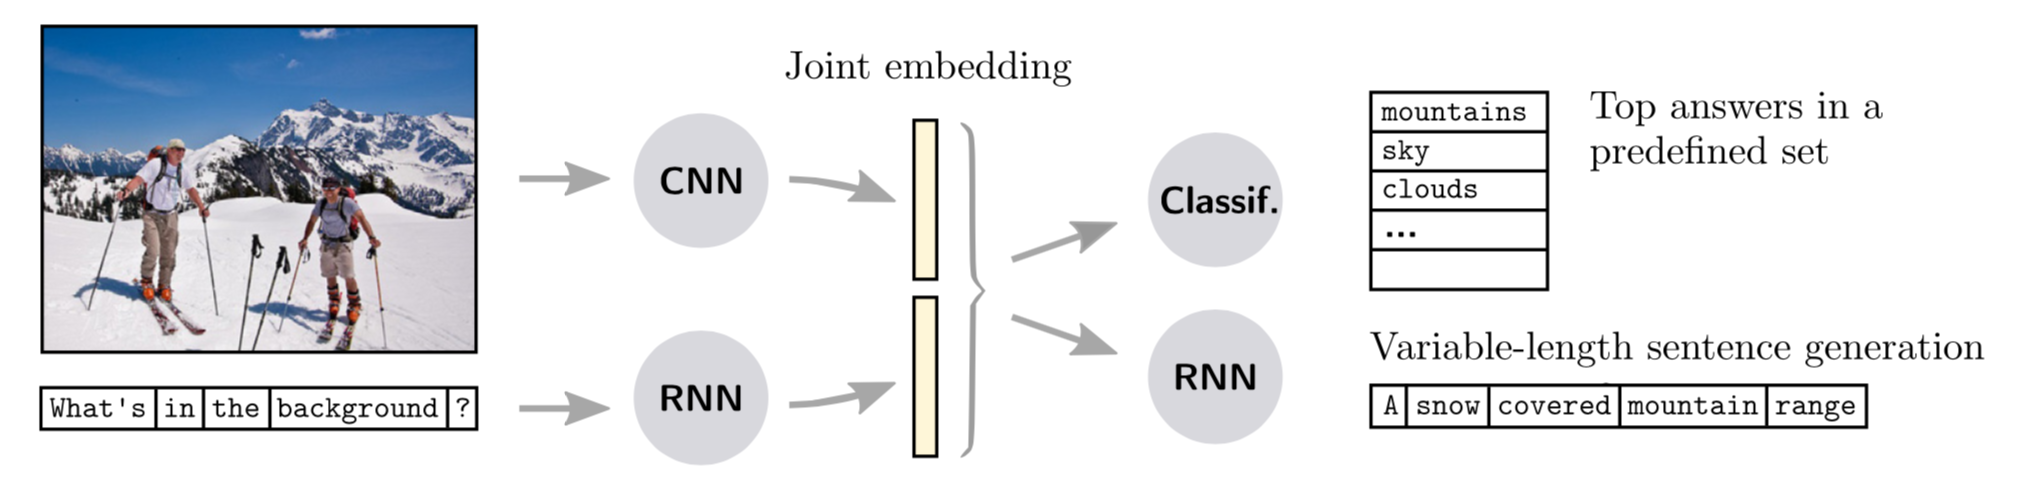
\includegraphics[width=0.8\textwidth]{answer-generation.png}
	\caption{常见的VQA方法是将图像和问题文本映射到同一特征空间,再组合融合两者的形成新的特征向量,特征向量作为分类器或者循环神经网络RNN(也可能是长短期记忆LSTM)的输入,输出得到最终的答案}
	\label{answer-generation}
\end{figure}

目前以神经网络为代表的基于分布式表示的机器学习算法核心思想都是寻找一种源数据和目标输出的“显著”的映射关系,例如在基于词嵌入的众多自然语言处理任务中,算法的目标都是寻找单词之间“显著”的搭配关系,从而完成句子补全或者问答任务;在图像识别等领域,同样的思想转化为寻找像素在二维甚至更高纬度的组合模式以表征物体对象。顺承这种模式匹配的思路,我们认为:所有视觉问答任务的答案在问题文本的统计分布和图像的统计分布之间存在强度的差异,而这种差异可以决定哪些信息对于回答问题更重要。所谓的统计分布的强度来源于人类相对稳定的行为模式下产生的数据,例如word2vec的不同的词嵌入在语义上存在的聚集性源,是因为这些词在训练数据中具有近似的上下文,而这种相似的语境产生于人类的语言习惯。我们提出以Q、q、I、i定性的表示“答案-问题强相关”、“答案-问题弱相关”、“答案-图像强相关”、“答案-图像弱相关”,从而组合得出四种问题类型QI、Qi、qI、qi,如表\ref{ques_type}所示。
\begin{table}[H]
% \resizebox{0.8\textwidth}{!}{}
\centering
\caption{根据答案和源信息的相关性划分出四类任务}
\begin{tabular*}{0.9\textwidth}{@{\extracolsep{\fill}}lccc}
\toprule
& \textbf{答案-问题相关性} & \textbf{答案-图像相关性} & \textbf{问题类型} \\
\midrule
\multirow{4}{*}{\textbf{相关性}} &  强& 强&  QI\\
&  强& 弱&  Qi\\
&  弱& 强&  qI\\
&  弱& 弱&  qi\\
\bottomrule
\end{tabular*}
\label{ques_type}
\end{table}

QI类型的问题需要同时结合图像特征和文本特征,这是一种最典型的视觉问答类型。Qi类型的问题答案可以直接根据问题文本得出,这类图像无关的问题可以退化为文本问答任务。qI类型的答案可以直接从图像中得出,这类问题退化为图像识别任务。例如,对于图\ref{DogExample},问题1:“图片中的狗是什么颜色?”,模型可以通过直接识别出图像中狗的色彩属性得出正确答案,那么问题1就是qI类型。对于同样的图片,问题2:“图片上的狗是不是属于动物?”是图像无关的Qi类型。
\begin{figure}[H]
	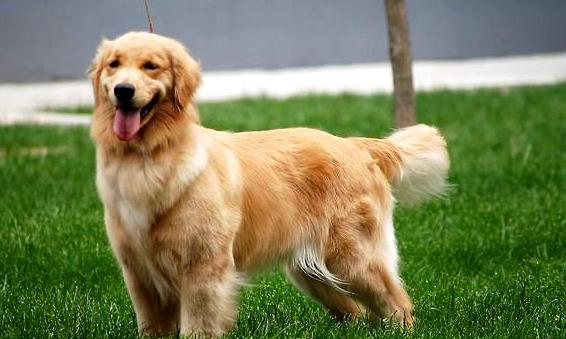
\includegraphics[width=0.8\textwidth]{DogExample.jpg}
	\caption{对于同一张图片,问题的不同将会决定模型是否需要外源知识或是常识。}
	\label{DogExample}
\end{figure}

qi类型的问题答案与问题文本和图像的相关性都比较弱,这类问题包含两类类型,一类为错误或者偏僻的问题,例如偏僻单词的问题、低频的语法结构;另一类为涉及常识和外源知识的问题,回答这类问题需要额外的知识,甚至还需要多步的推理,例如,对于图\ref{DogExample},问题3:“图片中的动物是什么颜色?”,模型除了需要正确识别图片中的狗和颜色属性,还需要知道“狗属于动物”的常识,才能在“狗的颜色”——黄色和“草地的颜色”——绿色之间做出正确的预测。目前,对于错误或者偏僻的qi问题研究较少,这类研究可以提升算法抗干扰能力,但不属于本文的研究内容。

但是值得注意的是,虽然视觉问答任务可以定性得细分为以上四个类型,但是上述分类标准是经验的。即使各个类型之间的边界是不够清晰的,这种划分方式也能帮助我们分析现有模型的侧重点,从而指导我们研究的方向。具体来说,现有的联合嵌入模型是将图像和文本特征融合训练,按照以上的划分标准,这些模型对QI、Qi、qI三种类型的问题有效的建模,但是无法回答qi类型。而基于知识库的模型便是希望引入额外特征从而解决弱问题和图像相关性的问题。

本节将简要介绍视觉问答方法中的联合嵌入模型和基于知识库的视觉问答方法,并且在联合嵌入模型的介绍中特别提出注意力机制和动态记忆网络两个部分。

\subsection{联合嵌入模型}
联合嵌入模型先将视觉信息和问题文本信息分别特征化,再通过特征向量串联\citing{zhou2015simple}、卷积\citing{ma2016learning}、逐元素相乘\citing{antol2015vqa}、逐元素相加\citing{malinowski2015ask}等池化方法融合图像特征和文本特征,最终得到最优答案。自从深度神经网络在计算机视觉和自然语言处理上的广泛应用以来,将各种模态的信息映射成特征向量的思想便大行其道,因此作为交叉领域中的视觉问答任务自然将多模信息联合嵌入到特征空间视为最“本能”的探索路径。

Malinowski等人首次提出了应用于真实场景视觉问答任务的联合嵌入模型Neural-Image-QA
\citing{malinowski2015ask}。Neural-Image-QA是一个由卷积神经网络CNN和长短期记忆LSTM组成的深度网络,先使用在ImageNet预处理过的卷积神经网络CNN对图像进行特征提取,得到的特征向量和问题文本一起传输到长短期记忆LSTM中,从而生成答案的单词序列。模型在DAQUAR数据集上完成训练和测试,对于答案只有一个词语的问题,准确率为19.43\%,对于答案是多个词语的问题,准确率为17.49\%。

Gao等人提出了mQA模型用于解决视觉问答任务\citing{NIPS2015_5641},mQA由四个部分构成,用于提取问题特征的长短期记忆LSTM(Q)、用于提取视觉特征的卷积神经网络CNN、用于存储具有多词的答案的语义上文的长短期记忆LSTM(A)、用于融合问题特征和已有的部分答案的语义特征并且预测答案的下一个词语的部分。提取视觉特征的CNN采用在ImageNet分类任务上预处理的卷积神经网络,在训练过程中保持不变,训练其他三个部分,以达到最高的准确率。区别于Malinowski的Neural-Image-QA,mQA认为问题和答案在句法结构上有所不同,因此编码问题的LSTM和解码答案的LSTM为采用两个独立的网络,使用不用的权重矩阵,为了降低系统过拟合的风险,共享了词嵌入层。整体架构如图\ref{mQA}。
\begin{figure}[H]
	\centering
	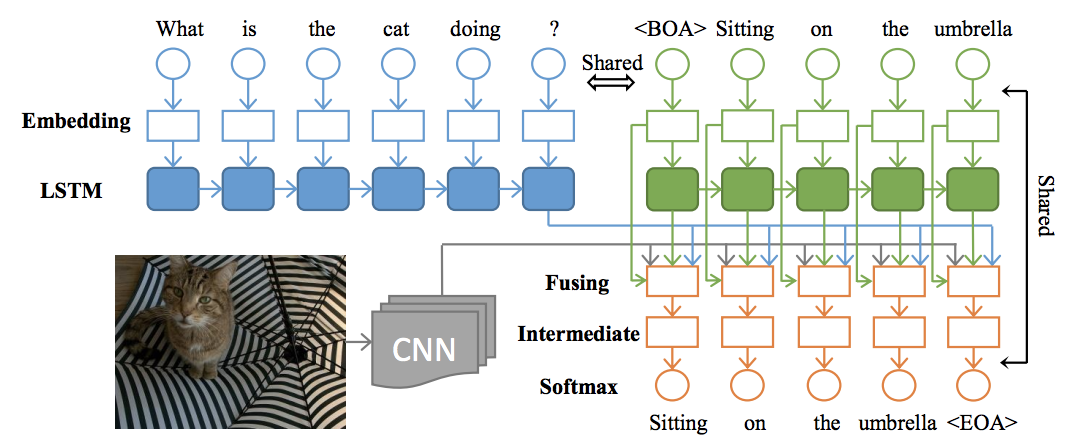
\includegraphics[width=0.8\textwidth]{mQA.png}
	\caption{mQA采用两个独立的LSTM编码问题序列和解码答案序列}
	\label{mQA}
\end{figure}

Noh等人认为单单使用相同权重参数的深度卷积神经网络去处理不同的问题,并期待能得到足够准确的答案,这是很困难的\citing{noh2016image}。因此他们提出DPPnet,在卷积神经网络CNN中添加一个动态参数层,动态参数层中的参数会根据问题的不同而改变,这使得每个问题输入都对应一个独特的分类网络。模型由三个部分组成,一个部分作为分类网络的卷积神经网络,第二个部分是参数预测网络,由门控复发单位编码问题序列,再通过一个全连接层输入动态参数,第三个部分是一个哈希函数,将参数预测网络输出的动态参数配置到分类网络中。如图\ref{DP-CNN}。
\begin{figure}[H]
	\centering
	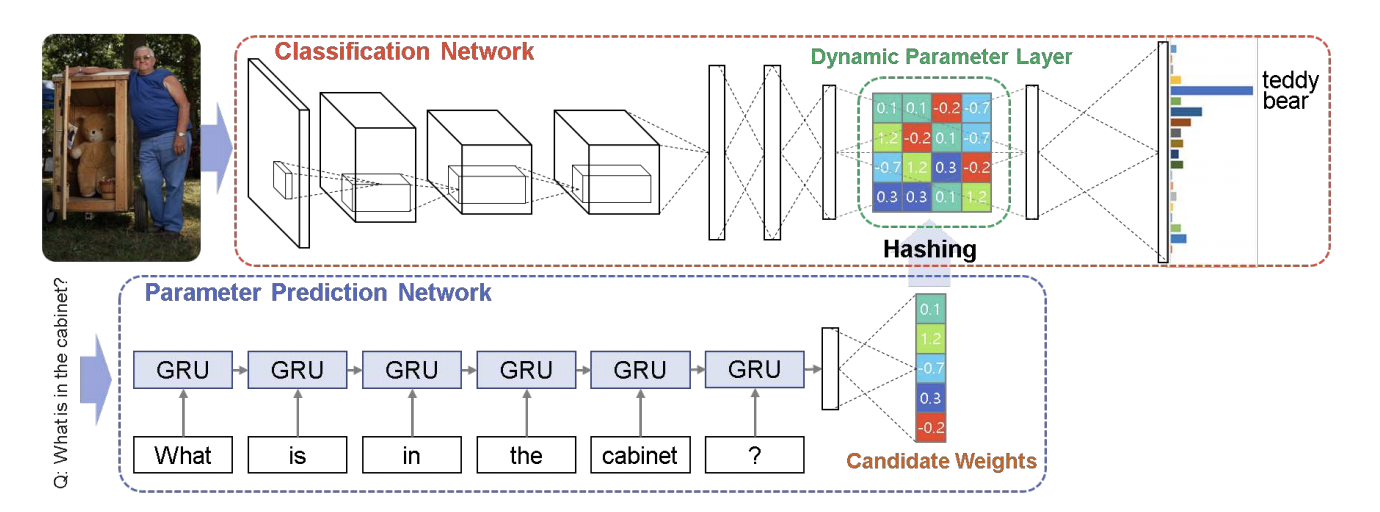
\includegraphics[width=0.8\textwidth]{DP-CNN.png}
	\caption{带有动态参数层的卷积网络模型DPPnet}
	\label{DP-CNN}
\end{figure}

Zhou等人同样适用预处理后的卷积神经网络CNN,但在处理问题文本时选择了比长短期记忆LSTM更为简单的词袋模型BOW,提出了iBOWIMG模型\citing{zhou2015simple}。iBOWIMG模型受到BOWIMG\citing{antol2015vqa}在VQA数据集上优于部分基于长短期记忆LSTM模型的启发,在原有基础上将VGGNet替换为在图像特征提取表现更优的GoogLeNet\citing{Szegedy_2015_CVPR},将图像特征向量和文本特征向量串联后送入softmax层预测问题答案(如图\ref{iBOWIMG}),在COCO-VQA数据集上的测试展现出具有竞争力的表现。
\begin{figure}[H]
	\centering
	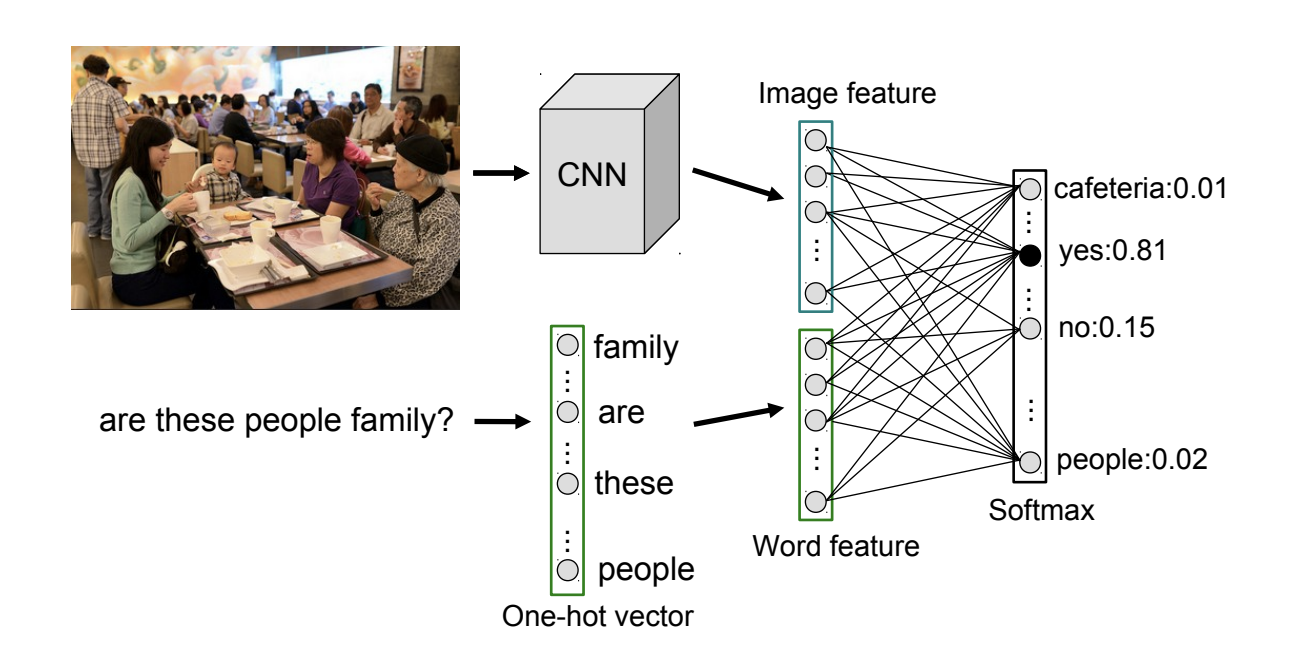
\includegraphics[width=0.8\textwidth]{iBOWIMG.png}
	\caption{iBOWIMG使用词袋BOW模型作为词特征向量编码器}
	\label{iBOWIMG}
\end{figure}

Lin等人将卷积神经网络CNN不仅应用于编码图像内容,而且也应用于问题文本的提取\citing{ma2016learning}。在处理图像特征和文本特征时使用一个多模态的卷积层输出联合特征向量,再使用softmax层预测最终的答案。如图\ref{lin}。
\begin{figure}[H]
	\centering
	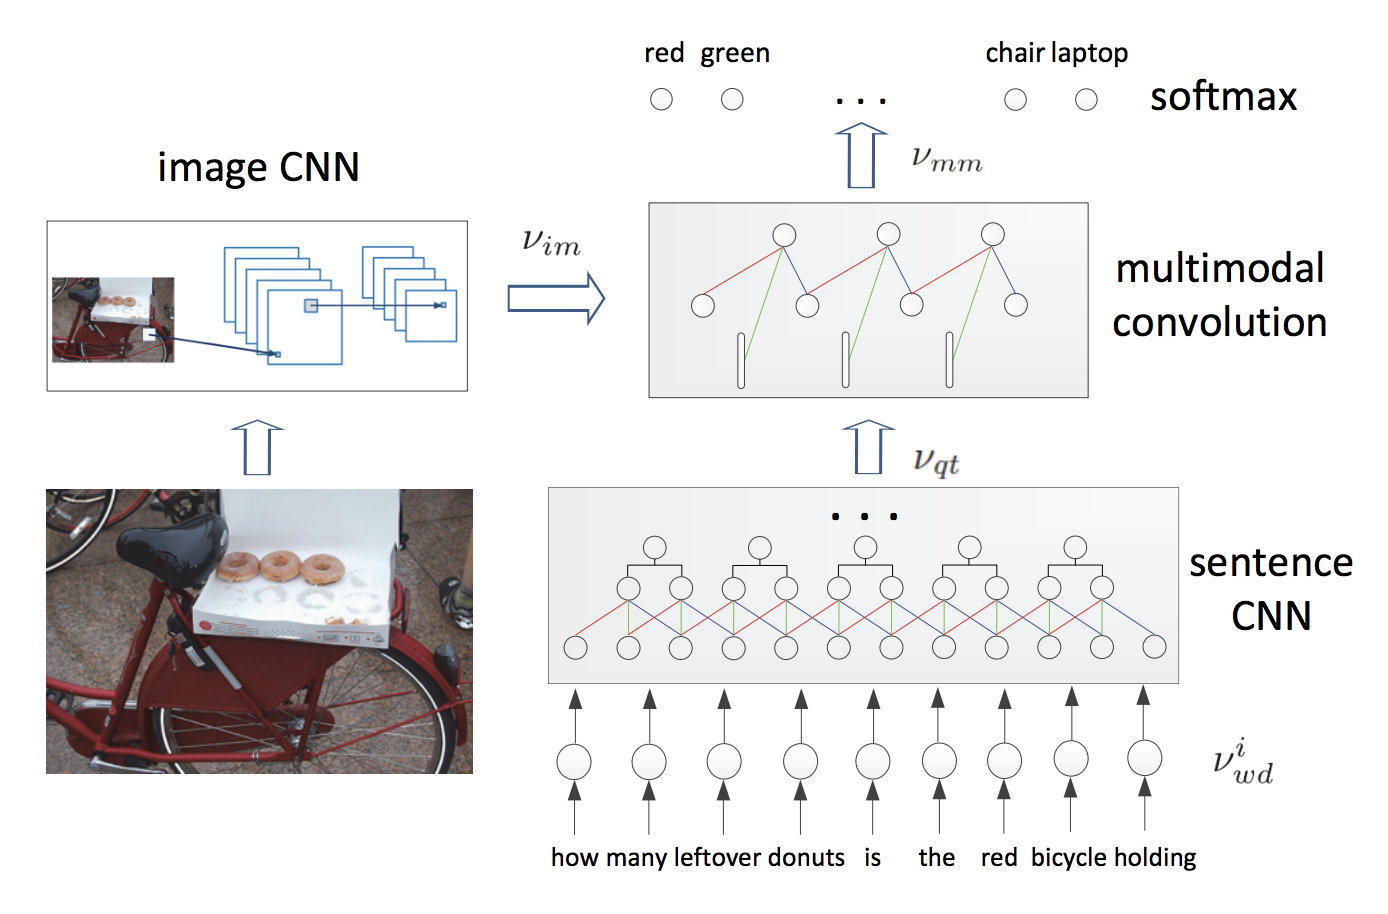
\includegraphics[width=0.8\textwidth]{lin.png}
	\caption{图像特征和问题文本特征提取时均使用CNN}
	\label{lin}
\end{figure}

除了使用不同的方法提取图像和文本特征以外,联合嵌入模型的另一个能够显著改善模型准确率的方向就是实验不用特征向量融合的池化方法。Malinowski等人通过对不同的特征向量融合方法的比较,可以看出系统的准确率与特征向量融合方法有关,不同方法之间准确率最多能相差9个百分点之多\citing{malinowski2015ask}。除了以上提到的iBOWIMG采用向量串联的方式,Lin使用向量卷积的方式外,Antol等人提出的模型使用逐元素相乘的方法融合两者\citing{antol2015vqa},Saito等人认为不同的特征融合方法各有特点,会保留或损失不同的特征,为了充分利用不同方法所保留的特征,提出了一种融合逐元素相加和逐元素相乘相结合的模型DualNet。模型同样利用了使用不同卷积神经网络CNN提取的图像特征,例如在真实场景图像采用了VGG-19\citing{simonyan2014very}、ResNet-152和ResNet-101\citing{he2016deep}。DualNet对提取出的文本特征和图像特征分别使用逐元素相加和逐元素相乘的方法得到两个不同的联合向量,再将两个的联合向量串联得到最终的合成向量,如图\ref{DualNet}。
\begin{figure}[H]
	\centering
	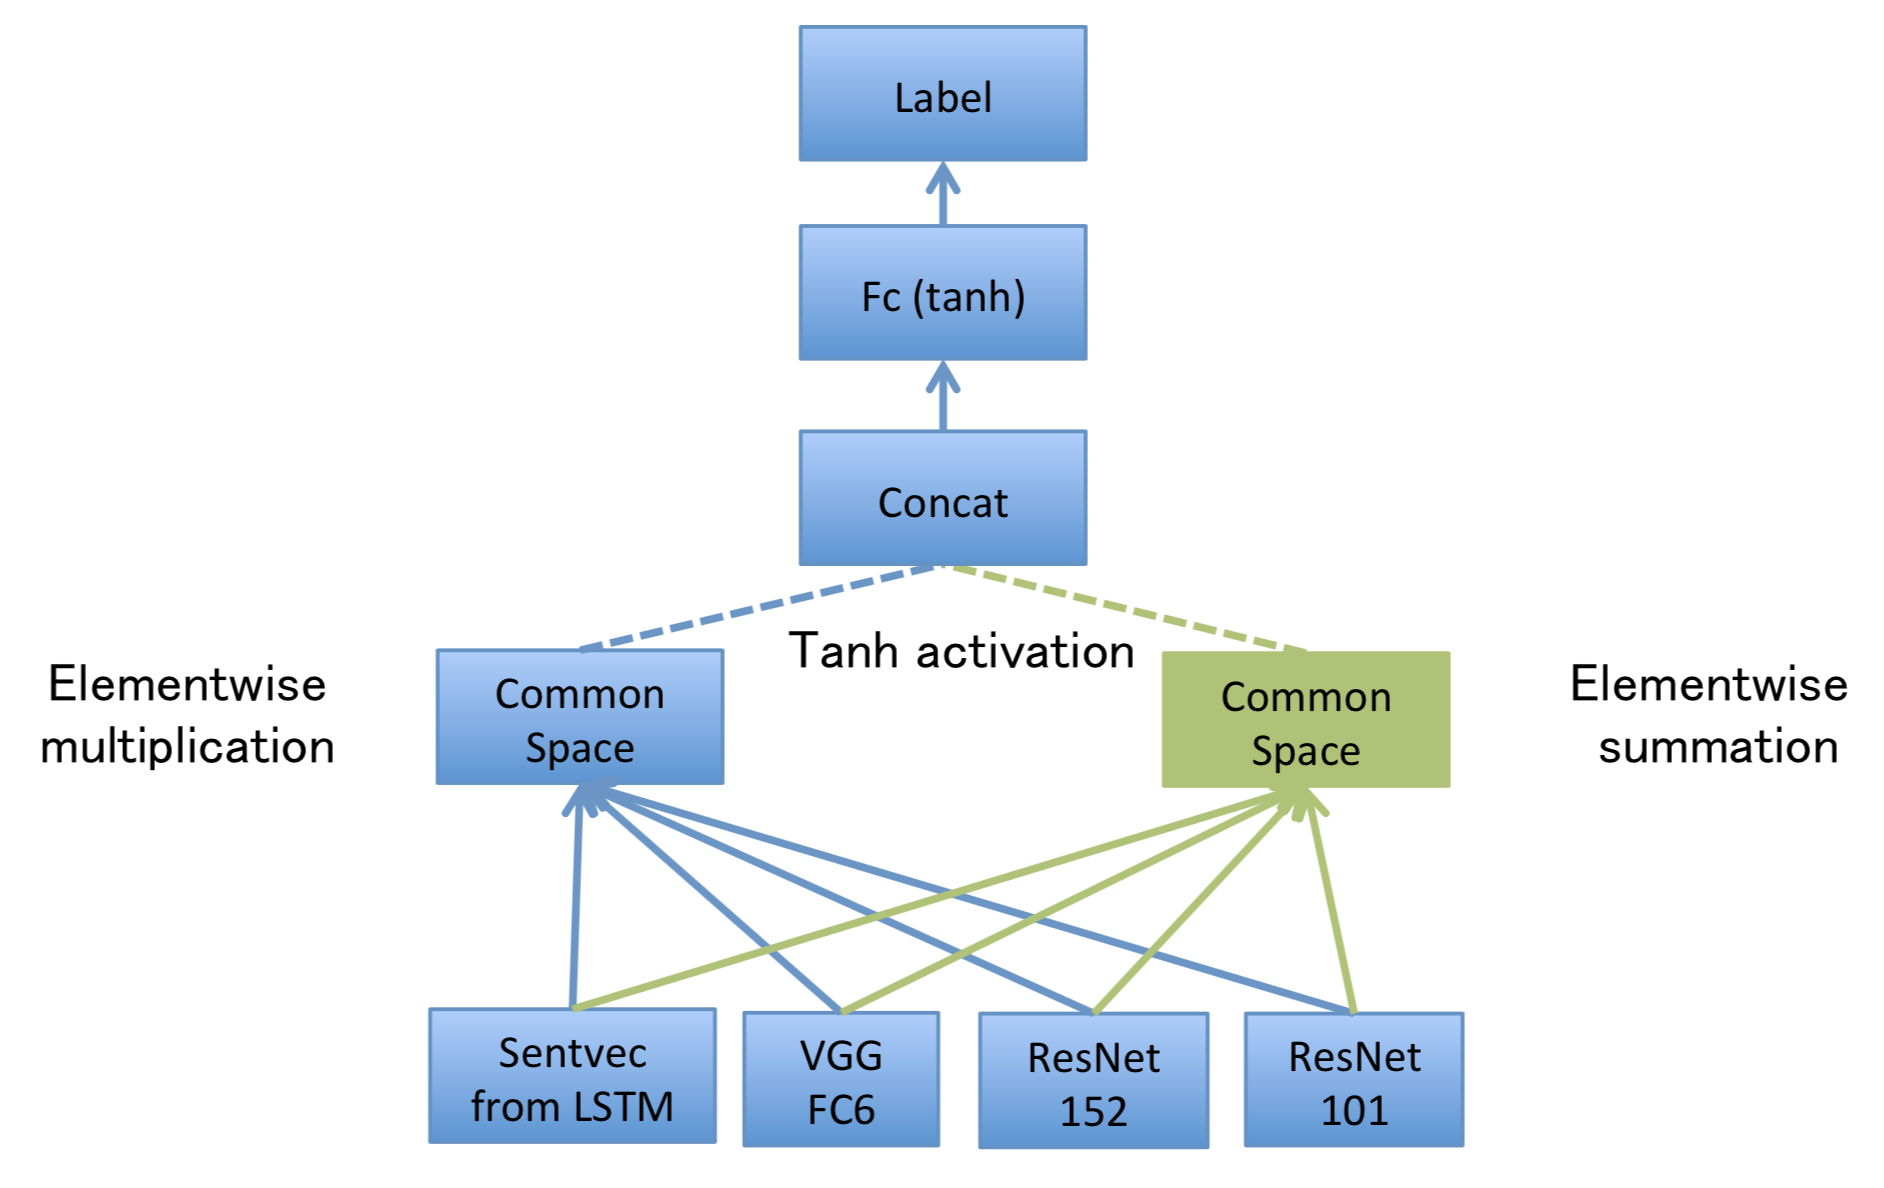
\includegraphics[width=0.8\textwidth]{DualNet.png}
	\caption{DualNet针对真实场景图像的模型架构}
	\label{DualNet}
\end{figure}

Fukui等人认为向量之间的外乘运算中,所有元素之间的互动更加活跃,应该能保留更加丰富的特征信息,因此提出一种更为复杂的多模态紧凑双线性池化方法(MCB)。一般的双线性模型会对两个向量的外乘结果线性化,外乘操作会得到异常高维的向量,例如外乘的两个向量维度均为2048、输出向量维度为3000时,那么训练参数的数量将达到125亿个之多,这会导致巨大的计算开销。而提出的多模态紧凑双线性方法能避免直接计算向量外乘,同时保留了大量特征,模型架构如图\ref{mcb}。
\begin{figure}[H]
	\centering
	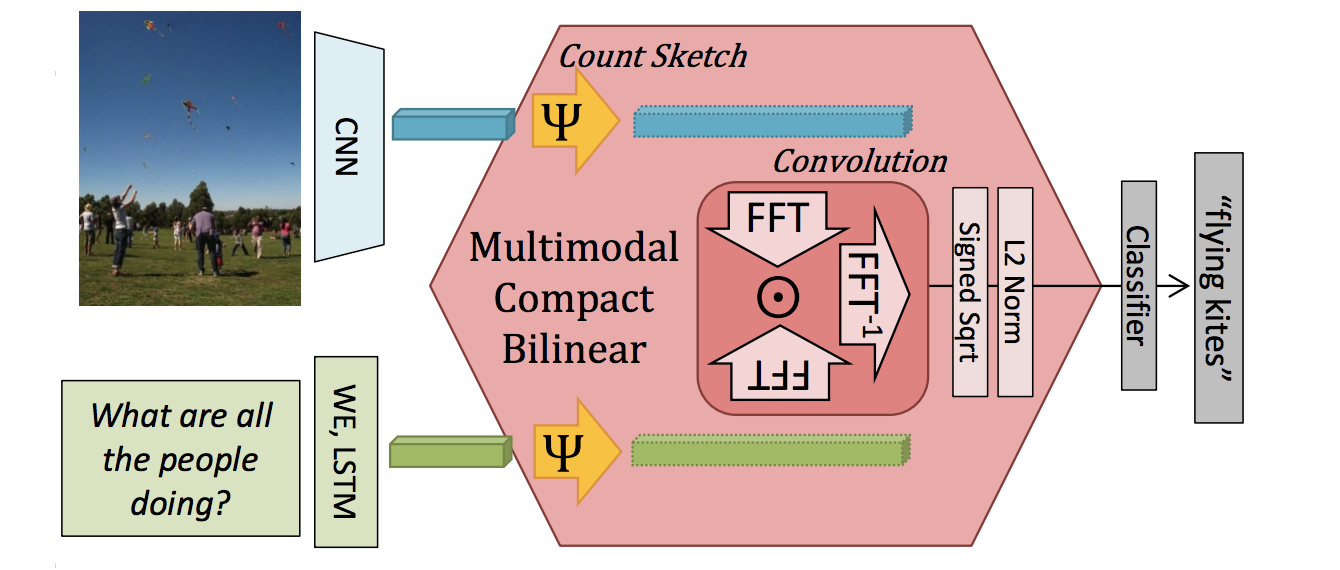
\includegraphics[width=0.8\textwidth]{mcb.png}
	\caption{使用多模态紧凑双线性池化融合图像和文本特征}
	\label{mcb}
\end{figure}

\subsubsection{注意力机制}
人类获取外部视觉信息时,会自动形成一种“像素不均衡”,在同一视野范围内的像素被视觉中枢神经系统根据“关注区域”的远近、相关性特征自动分配不同的分辨率,使得“关注区域”内的像素具有极高的分辨率,而其他的像素仅仅作为视觉信息输入,并不参与大脑的语义处理(如图所示\ref{human-virtual})。因此视觉注意力机制帮助大脑过滤了低相关性的视觉信息,减少了待处理数据的体积,极大地提高了信息处理速率并松弛了大脑负载。
\begin{figure}[H]
	\centering
	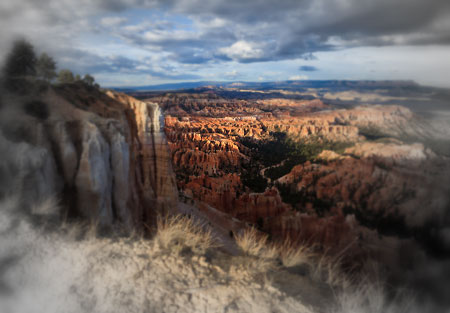
\includegraphics[width=0.5\textwidth]{human-virtual.png}
	\caption{人类视觉系统的“像素不均匀”现象}
	\label{human-virtual}
\end{figure}

近几年,受到人类视觉注意力机制的启发,在神经网络中引入注意力机制变得十分热门,在自然语言处理和计算机视觉领域的应用也极大得帮助了原有算法精度和计算效率的提升。Google Deepmind团队提出了一种带有注意力机制的循环神经网络(RNN),并成功应用于图像分类任务,获得了优于以往卷积神经网络(CNN)的基线水平的分类精度\citing{mnih2014recurrent}。随后,带有注意力机制的循环神经网络便被广泛应用于自然语言处理和计算机视觉的多个子领域\citing{bahdanau2014neural, xu2015show, NIPS2015_5847}。Bahdanau等人将注意力机制引入神经机器翻译任务,仍然使用“编码-解码”的翻译模式,但一改以往将源语言文本映射为一个固定长度的向量的编码方式,而是将原语言文本编码为向量序列,解码时将翻译和位置对应因素联合学习,训练向量序列中各向量对翻译词组的不同权重,加和完成翻译结果的推断,得到了以往最优的结果\citing{bahdanau2014neural}。Xu等人受到注意力机制在机器翻译和物体识别任务成功应用的启发,将带有注意力机制的循环神经网络应用于自动生成图像标注,并且在Flickr9k, Flickr30k 和MS COCO 三个数据集上均获得了最优的结果\citing{xu2015show}。随后,更多注意力机制的变型或优化研究均在图像标注任务上展开\citing{ 7243334, wu2017global, li2017image, lu2017knowing}。

相较起图像标注任务,视觉问答任务除了要求系统能理解图片内容,生成语义和句式合理的自然语言文本以外,还需要联合学习问题文本和聚焦与问题相关的图像细节。这些任务特性决定了视觉问答任务可以利用已有较为先进的图像标注任务的框架,同时融合自然语言处理的最新成果。注意力机制在自然语言处理和计算机视觉上的成功应用便成为了视觉问答算法快速发展的基石。

Chen等人最先将注意力机制引入视觉问答任务,提出了基于注意力机制的可配置卷积神经网络(ABC-CNN)用于针对“图像问题对”生成对应的注意力映射,将问题的语义信息和图像区域建立映射,使得答案生成取决于被关注区域,减少无关区域的影响\citing{chen2015abc}(模型架构如图\ref{abc-cnn})。在Toronto COCO-QA\citing{ren2015exploring}, DAQUAR\citing{ malinowski2014multi}, 和VQA\citing{antol2015vqa}三个数据集上的测试结果都提升了最优结果,证明了注意力机制在提高视觉问答任务上的有效性,同时注意力权重图能反应系统的推理过程,为参数的微调提供了依据。
\begin{figure}[H]
	\centering
	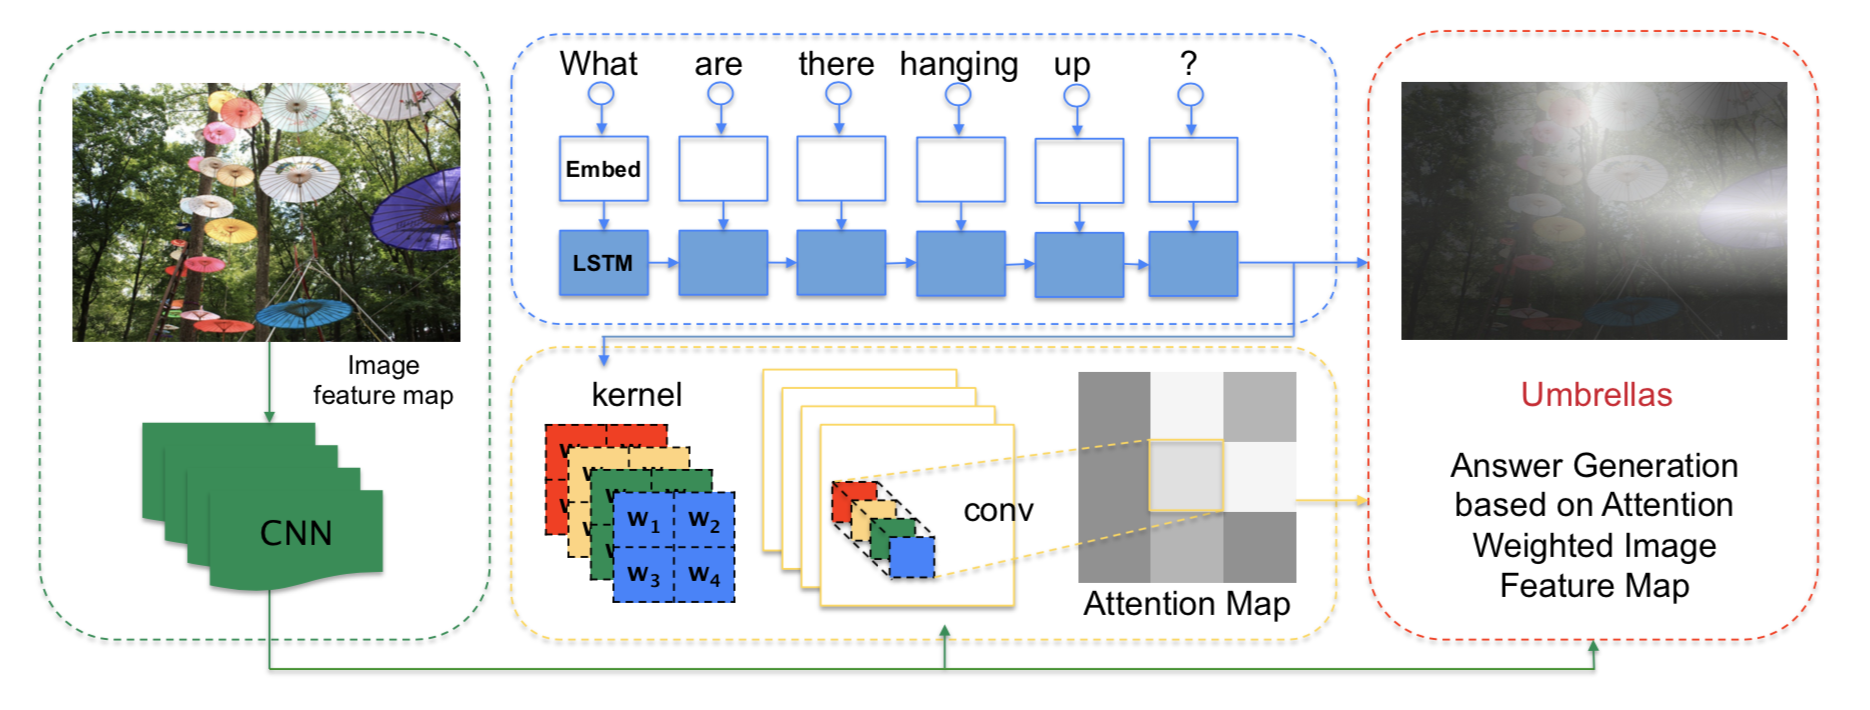
\includegraphics[width=0.8\textwidth]{abc-cnn.png}
	\caption{ABC-CNN使用CNN提取图像特征,LSTM提取问题文本特征,黄色方框内为用于推测与问题相关的图像区域的注意力机制}
	\label{abc-cnn}
\end{figure}

Shih等人使用简单的word2vec方法编码“问题-答案”对,使用预处理后的卷积神经网络CNN对图片的不同区域编码,将编码后的文本特征向量和图片特征向量映射到同一特征空间,根据特征之间的点乘运算决定每个图像区域的权重,最后结合权重化以后的图像特征和文本特征得出答案。架构如图\ref{shih}。在辨别物体颜色的任务上得到了最优结果\citing{ shih2016look}。类似的工作还有Ilievski等人提出的“聚焦型动态注意力模型“\citing{ilievski2016focused}。
\begin{figure}[H]
	\centering
	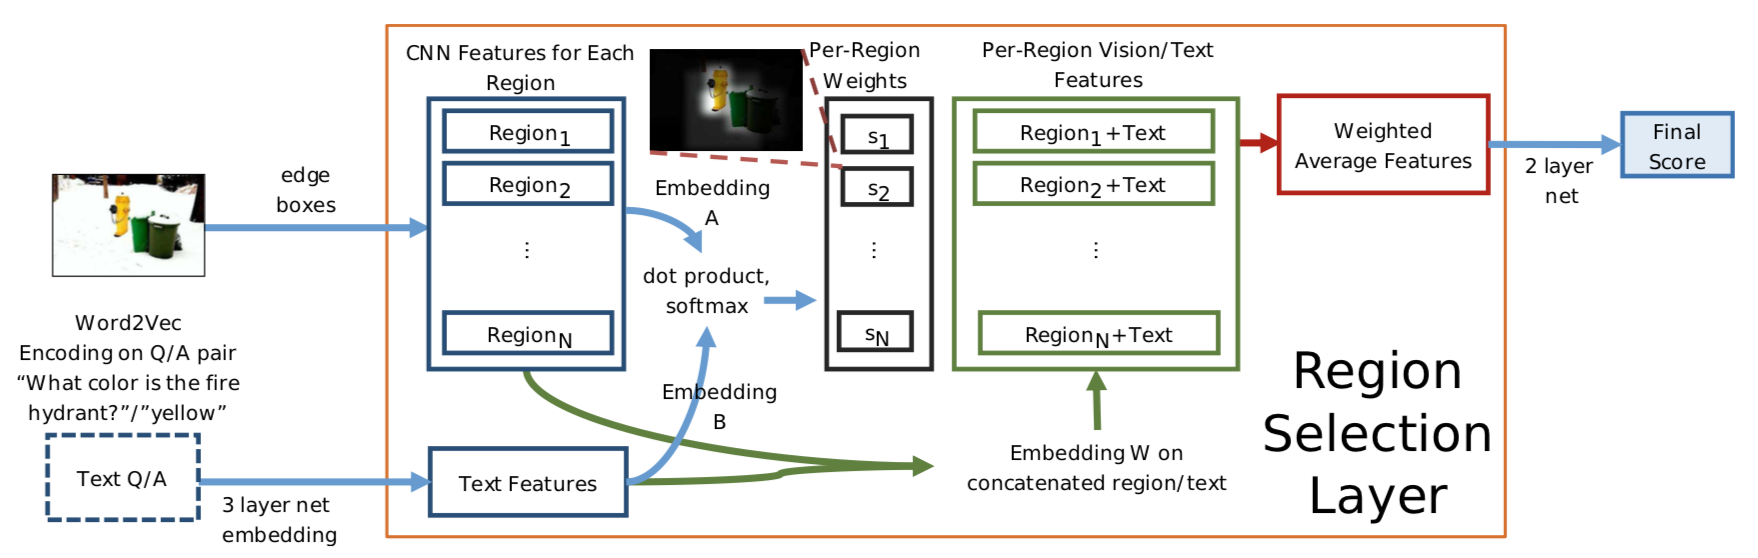
\includegraphics[width=0.8\textwidth]{shih.png}
	\caption{使用图片区域选择层实现注意力机制的架构}
	\label{shih}
\end{figure}

包括以上提到的在内,多数注意力机制对问题文本和图像区域特征进行一次运算,直接生成图像注意力权重图。针对这种情况,Yang等人提出堆栈式注意力网络——使用问题的语义表达对图像进行多次查询,不断缩小答案相关区域,实现更高的精度\citing{yang2016stacked}。注意力机制在视觉问答上的其他应用还有,同时使用对图像和问题使用注意力机制的联合注意力模型\citing{NIPS2016_6202};不采用图像区域赋值方法,而是过滤掉不相关区域的“自适应硬性注意力网络”\citing{malinowski2018learning}。

对于神经网络训练这类参数密集和计算密集的框架,注意力机制能带来两个重要的改变。一方面,无论对于图像输入还是文本输入,原有的方法都选择将输入看做一个整体,因此映射后的向量需要包含完整的输入信息,对于包含词组过多文本或是场景过于复杂的图像,编码后的向量根本无法区分开输入的局部特征,这使得神经网络的可解释性大大降低。引入注意力机制后,编码方式改变,将输入视为为局部信息的综合,保留了文本中单词和图像中像素区域的信息,通过可视化处理,能清晰的看出神经网络的推理过程,增强了系统的可解释性,可以称之为一种“弱化黑盒的处理”。另一方面,注意力机制非常符合人类对于语言和视觉信息的处理方式,这背后的假设是:针对绝大多数任务,只需要从信息源的局部便能获得充分正确的答案。类似于人类,具有注意力机制的智能体应当能获得更高的执行的效率和更高的答案精度。

\subsubsection{动态记忆网络}
无论是在自然语言理解还是图像内容理解,人类在获取单词或者图像像素区域的语义时不会将其与语境割裂来看,通常上下文语境对于准确理解文本和图像信息是非常重要的,因为在语言和图像中存在大量具有歧义特性的内容,例如,在语言中一个单词具有不同的语义,也可能有不同的词性,只有在上下文的语境中才能确定词语的真正含义。记忆力与上下文语境相似,是神经网络在训练过程中存储的“经验”,这种“经验”有助于以后的训练,这种累积经验能创造更准确的答案,基于这样的假设,研究人员为从序列化的输入中获得更准确的输入,而引入了动态记忆网络\citing{jiang2015compositional,kumar2016ask,xiong2016dynamic}。

Jiang等人在常见的CNN解析图像、LSTM解析问题文本的架构上,新增一个成分记忆模块\citing{jiang2015compositional},旨在融合每一次训练过程中的局部图像信息和文本信息,并提供给下一次训练使用,从而使网络存储了训练过程的“经验”,这与之后提出的动态记忆网络有同样的思想,模型训练流程如图\ref{c-memory}。
\begin{figure}[H]
	\centering
	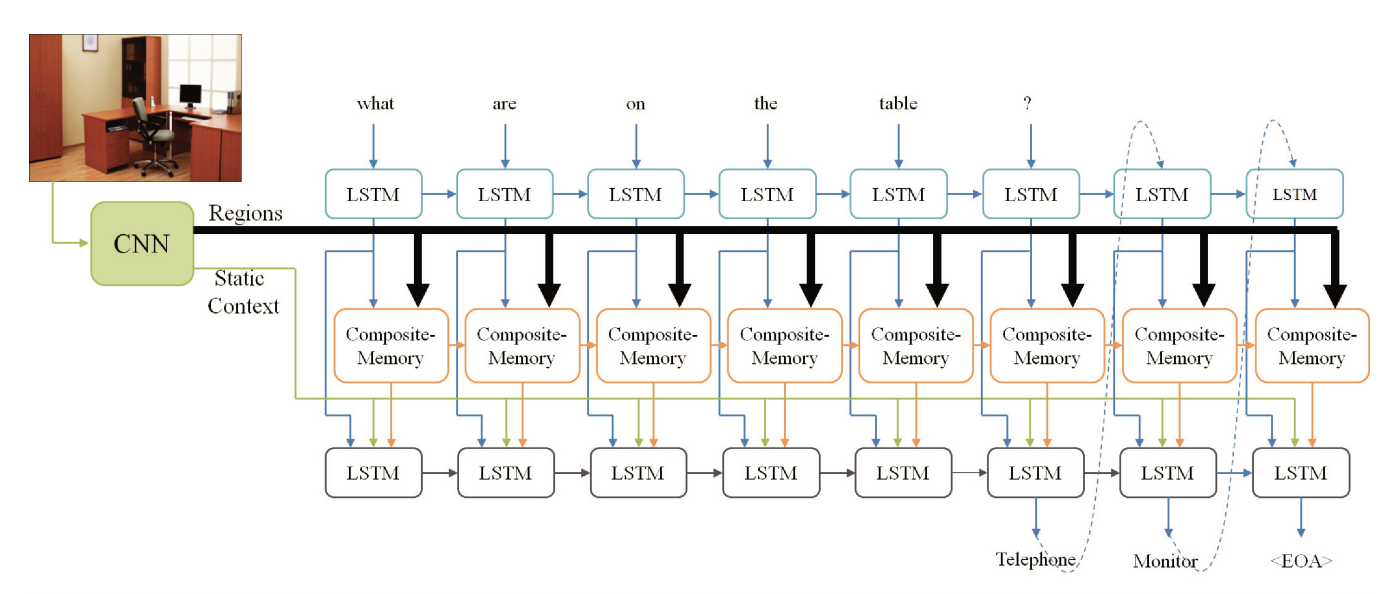
\includegraphics[width=0.8\textwidth]{c-memory.png}
	\caption{成分记忆模型的训练流程}
	\label{c-memory}
\end{figure}

Kumar等人为解决文本问答(Text-QA)任务而提出动态记忆网络(DMN)\citing{kumar2016ask}。动态记忆网络(DMN)是一个用于生成文本问题答案的神经网络框架,它由输入模块、问题模块、情节记忆模块和问题模块构成,输入模块用于编码文本输入;问题模块用于编码文本问题;情节记忆模块接受由输入和问题模块得到的分布式向量,再使用注意力机制选择部分接受到的向量,结合选择后的向量与以往存储的“记忆”生成新的“记忆”向量,并不断迭代;答案模块根据最终的记忆向量生成答案,模型架构如图\ref{dmn}。
\begin{figure}[H]
	\centering
	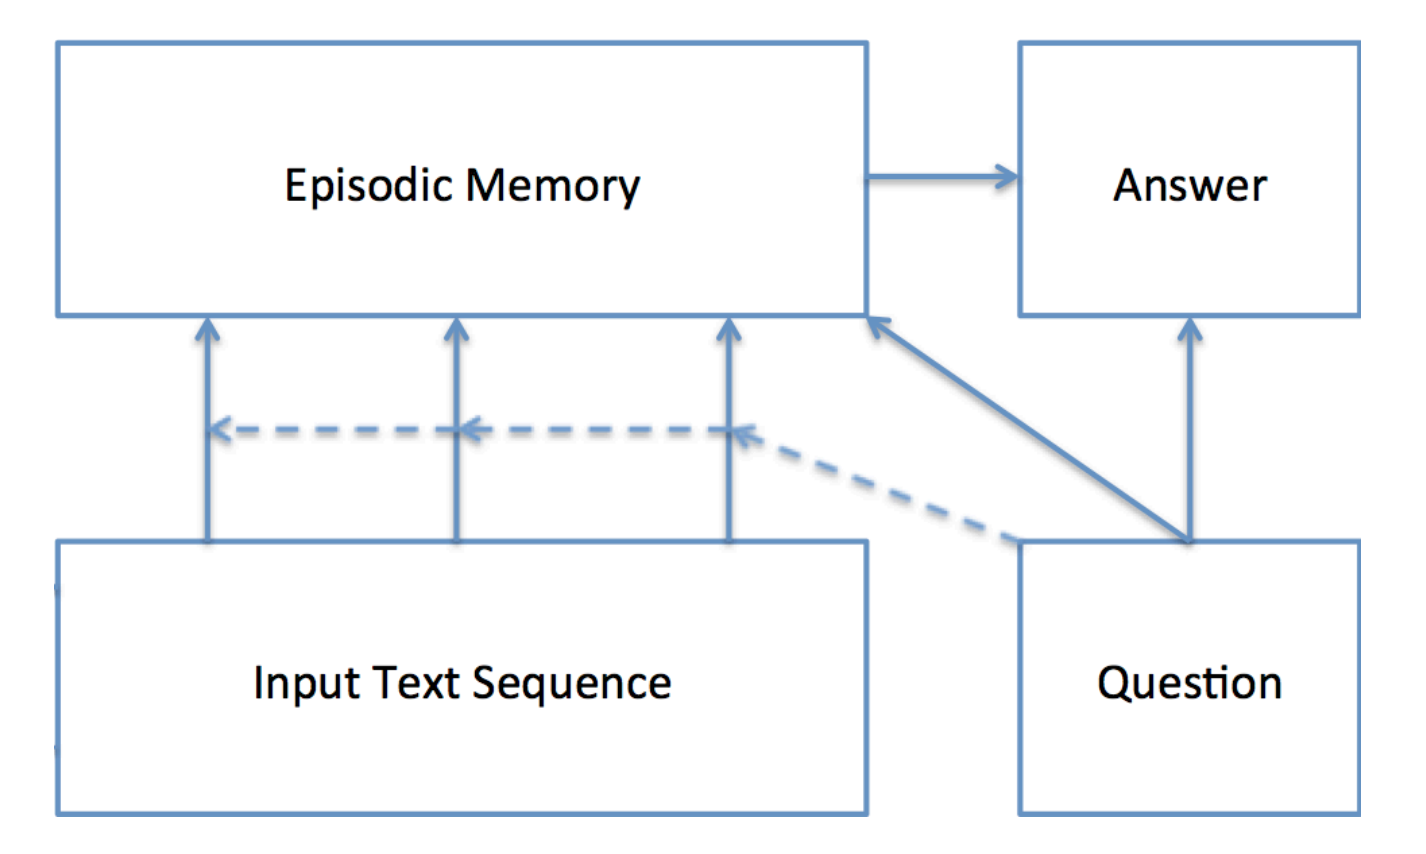
\includegraphics[width=0.5\textwidth]{dmn.png}
	\caption{DMN基础架构}
	\label{dmn}
\end{figure}

动态记忆网络(DMN)在文本问答、语义分析、词性标注任务上取得了最优的结果,受到其在处理序列化的文本信息上的优异表现的启发,Xiong等人在原有网络的基础上改善了输入和记忆模块,除了能处理文本信息外,还能处理图像信息,提出应用到于视觉问答任务动态记忆网络+(DMN+)\citing{xiong2016dynamic},如图\ref{v-dmn}。动态记忆网络+(DMN+)将原有的输入模块中处理文本编码的门控复发单元(GRU)更换为双向门控复发单元(bi-GRU)以得到文本或图像区域更完整的上下文信息;使用基于注意力机制的门控复发单元替换原有的软性注意力机制。更新后的动态记忆网络+(DMN+)在DAQUAR\citing{malinowski2014multi}和VQA数据集\citing{antol2015vqa}上的测试结果都得到了具有竞争力的表现。
\begin{figure}[H]
	\centering
	\subfigure[应用于文本问答的动态记忆网络(DMN)模型架构]{
		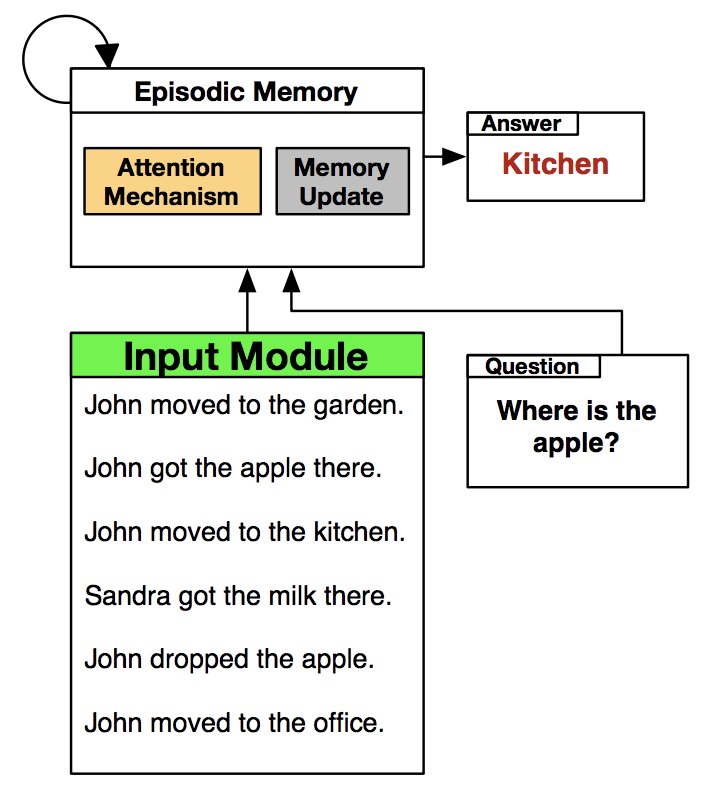
\includegraphics[width=0.4\textwidth]{t-dmn.png}}
	\subfigure[应用于视觉问答的动态记忆网络+(DMN+)模型架构]{
		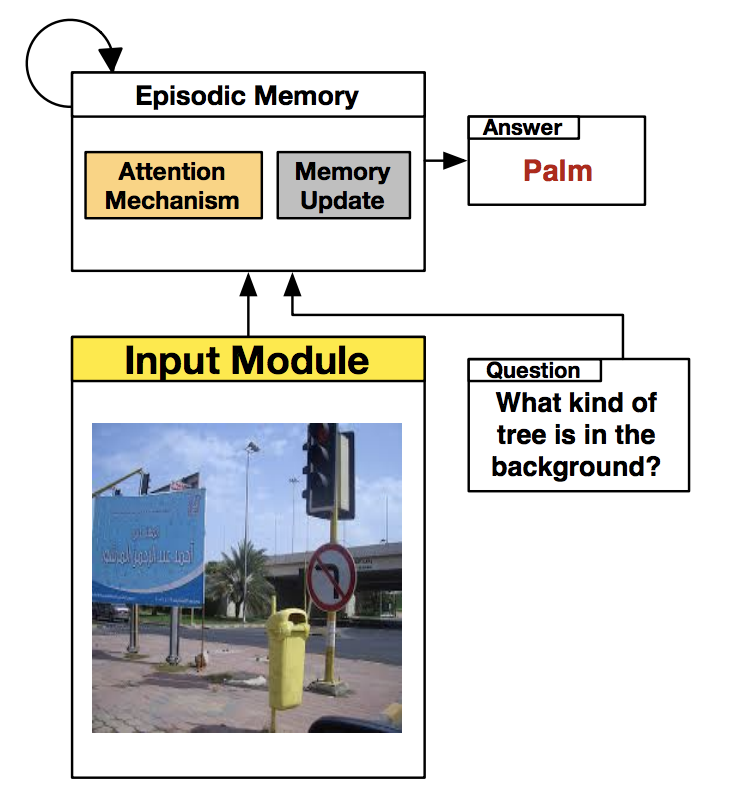
\includegraphics[width=0.4\textwidth]{v-dmn.png}}
	\caption{DMN+与DMN架构对比}
	\label{v-dmn}
\end{figure}

\subsection{基于外源知识库的视觉问答算法}
视觉问答任务基于图像场景回答问题,图像理解、问题理解和答案生成是实现准确的视觉问答系统的算法核心。图像理解、问题理解和答案生成三者又可以根据人类思考逻辑将其划分为两个逻辑层次,问题理解成为逻辑基点,图像理解和答案生成都根据问题的不同而采用适当的算法策略——注意力机制便是一种借助问题理解而实现计算效率更高的图像解析方法,答案生成中关心的答案类型和答案词组长度也需要依照问题的不同而选择。因此问题的解析过程对于视觉问答算法的准确性和计算成本都有很大的影响。

正如绪论中提及的,问题可以分为识别和推理两个大类,推理任务中既要求系统能准确识别图像中的对象,往往也会涉及图像中无法获取的先验知识。先验知识包括众所周知但不会显性呈现的常识和面对特定领域需要具备的专业知识,例如,判断路口是否可以通行时,涉及基本交通规则的常识,判断艺术品的作者这类专业问题时,需要借助与该艺术品相关的知识储备。

先验知识对视觉问答系统提出了更高的要求,这也揭露了主流的联合嵌入模型的缺陷:第一点,联合嵌入模型的答案生成来源于训练集中的问题和答案文本,这意味着训练集中包含的知识和文本内容是整个视觉问答系统的所有知识来源,因此对于测试集中涉及的全新概念或答案,系统根本无法得出正确的答案。不断扩充包含更多先验知识的训练集是提高精度的方式之一,但对于整个世界蕴含的不可计量的知识而言,这种数据集扩充的方式成本巨大。第二点,联合嵌入模型要求网络本身能存储学习到的知识,目前网络的容量相较于需要学习的知识是严重不足的。第三点,神经网络海量参数和复杂网络连接带来的黑盒特性依然存在。对于识别和分类等问题而言,可解释性与高精确度相比,显得不那么重要,但是对于需要明确推理过程的问答系统而言,黑盒的不可解释性会降低提问者对系统的可信度,毕竟没人会轻易相信一个无法解释的答案。

一种可行的解决方案是将推理过程和知识学习分离,保留系统原有的图像理解和问题文本理解模块,在答案生成模块中引入外源知识库。可扩展的外源知识库可以解决网络容量的限制问题;知识库中结构化的数据可以作为推理过程的起点,知识库中的数据关联能为推理提供路径,形成逻辑链条,提高系统的可解释性。本节将对已有的基于知识库的视觉问答方法进行详细的介绍,分析各种方法的优势和存在的问题。

\textbf{Ahab}

Wang等人提出的Ahab视觉问答系统利用DBpedia作为知识库,实现对需要先验知识的问题的推理应答,即使问题中涉及不包含于图像中的概念\citing{wang2015explicit}。Ahab的主要思路为三点,第一点,将图像中的概念链接到知识库中相同的概念,形成从图像到知识库的映射,第二点,将自然语言的文本问题处理为知识库查询语句,实现从自然语言的句法和语义结构变换到相应的查询语句结构,第三点,将知识库的查询结果转换为自然语言表达。利用以上三点,Ahab可以不通过数据集训练获取知识,而使用自然语言到知识库的两次转化完成问答任务。

具体来说,为了建立图像概念到知识库实体之间的映射,首先检测图像包含的概念,再将提取出的图像概念和知识库实体建立链接。Ahab从图像中提取物体对象、图像场景和图像属性三种视觉概念,对象提取使用在MS COCO\citing{lin2014microsoft}和ImageNet\citing{deng2009imagenet}上预训练后的Fast-RCNN\citing{ren2015faster},能实现224种类型的对象识别;场景分类器使用预处理于MIT Places205\citing{zhou2014learning}数据集的VGG-16 CNN,理论上能实现对205种场景的识别,每张图片选取分数前三的场景标签;图像属性提取器使用预处理于ImageNet\citing{deng2009imagenet}和MS COCO\citing{lin2014microsoft}的VGG-16 CNN,每张图片选取分数前十的属性标签。所有提取出的图像信息都使用资源描述框架(RDF)的形式表示,例如,“图像中包含长颈鹿对象”被表示为(图像,包含,对象1),(对象1,名称,长颈鹿)。每个视觉概念则被直接链接到具有相同语义的知识库概念,如图所示\ref{linkingMathord}。
\begin{figure}[H]
	\centering
	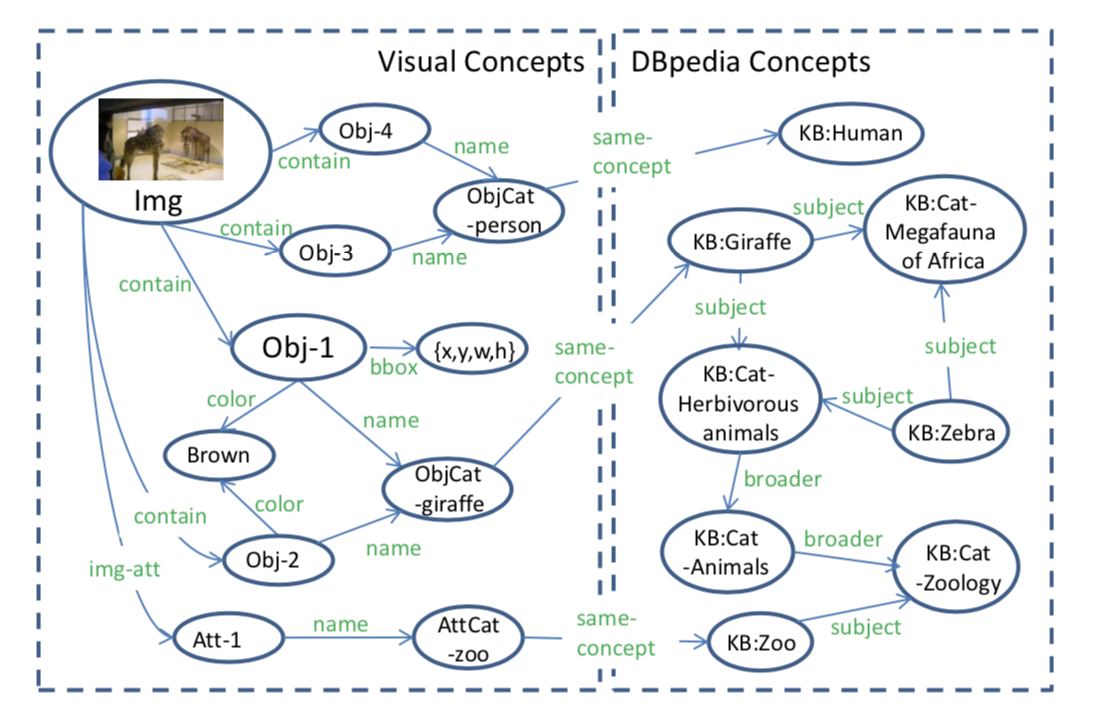
\includegraphics[width=0.8\textwidth]{linkingMathord.png}
	\caption{Ahab中链接图像信息和知识库实体的RDF图结构}
	\label{linkingMathord}
\end{figure}
所有资源描述框架(RDF)数据被存储在OpenLink Virtuoso中——一个能存储多种数据类型的数据库。

Ahab使用Quepy开源框架将自然语言问题转化为相应的知识库查询语句,但Quepy解析问题时,需要预先设定的正则表达式模板,因此Wang等人使用KB-VQA数据集作为实验数据集。结合KB-VQA中的23种问题模板和针对不同问题类型的谓语选择,Ahab能根据不同的问题产生相应的查询语句,并得到问题答案。

Ahab类似于专家系统,针对特定的问题设定了与之对应的知识库查询方法,应用于知识库的搜索路径可以为视为系统“逻辑推理”的过程,因此Ahab不仅输出最终的答案,而且也将答案推理的过程作为输出,实现了对系统推理的显性表达,问题处理的过程如图\ref{question_processing}。
\begin{figure}[H]
	\centering
	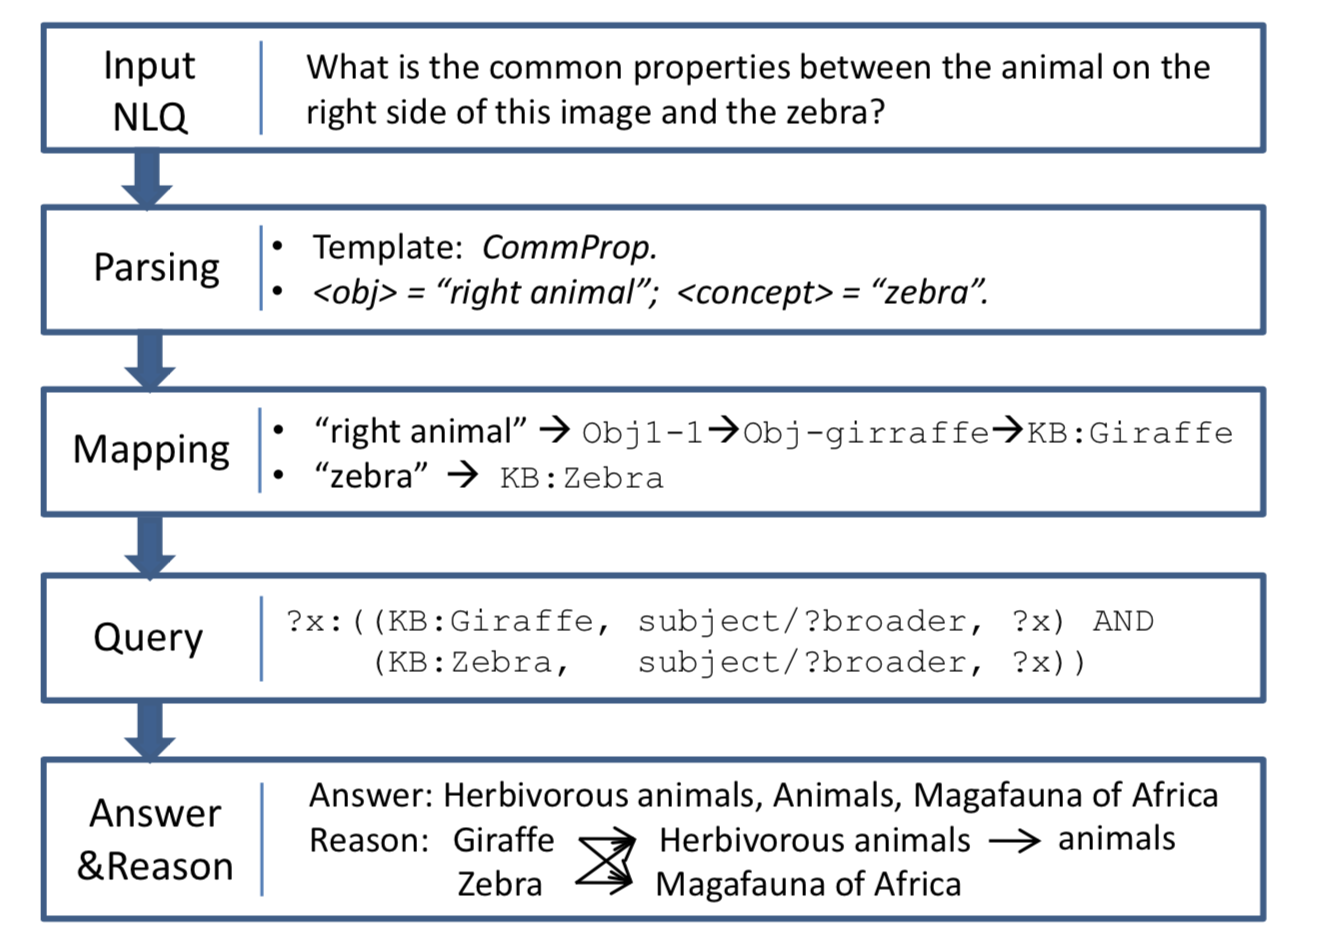
\includegraphics[width=0.8\textwidth]{question_processing.png}
	\caption{Ahab结合问题文本和预先设定的模板,解析出问题中的概念,再将问题中的概念与知识库实体建立链接,并生成查询语句,得到查询结果和推理过程}
	\label{question_processing}
\end{figure}

在评估Ahab对于需要先验知识的问题的表现时,Wang等人使用了自己构建的KB-VQA数据集\citing{wang2015explicit}作为测试集,但KB-VQA中的问题多数是开放性的,并且还没有自动化评估正确性的方法被提出,因此使用人工的方式对结果的正确性进行评估,每个结果被人工地赋予5种表示正确程度的分数:1分-完全错误、2分-部分错误、3分-模棱两可、4分-基本正确、5分-完全正确。

作为对比,评估还引入了由人类作答和主流的联合嵌入模型作答两种方式——使用CNN编码图像特征,LSTM编码问题文本和生成答案的模型,三种测试系统在不同问题的正确率和平均得分如图\ref{ahab_evaluation}。
\begin{figure}[H]
	\centering
	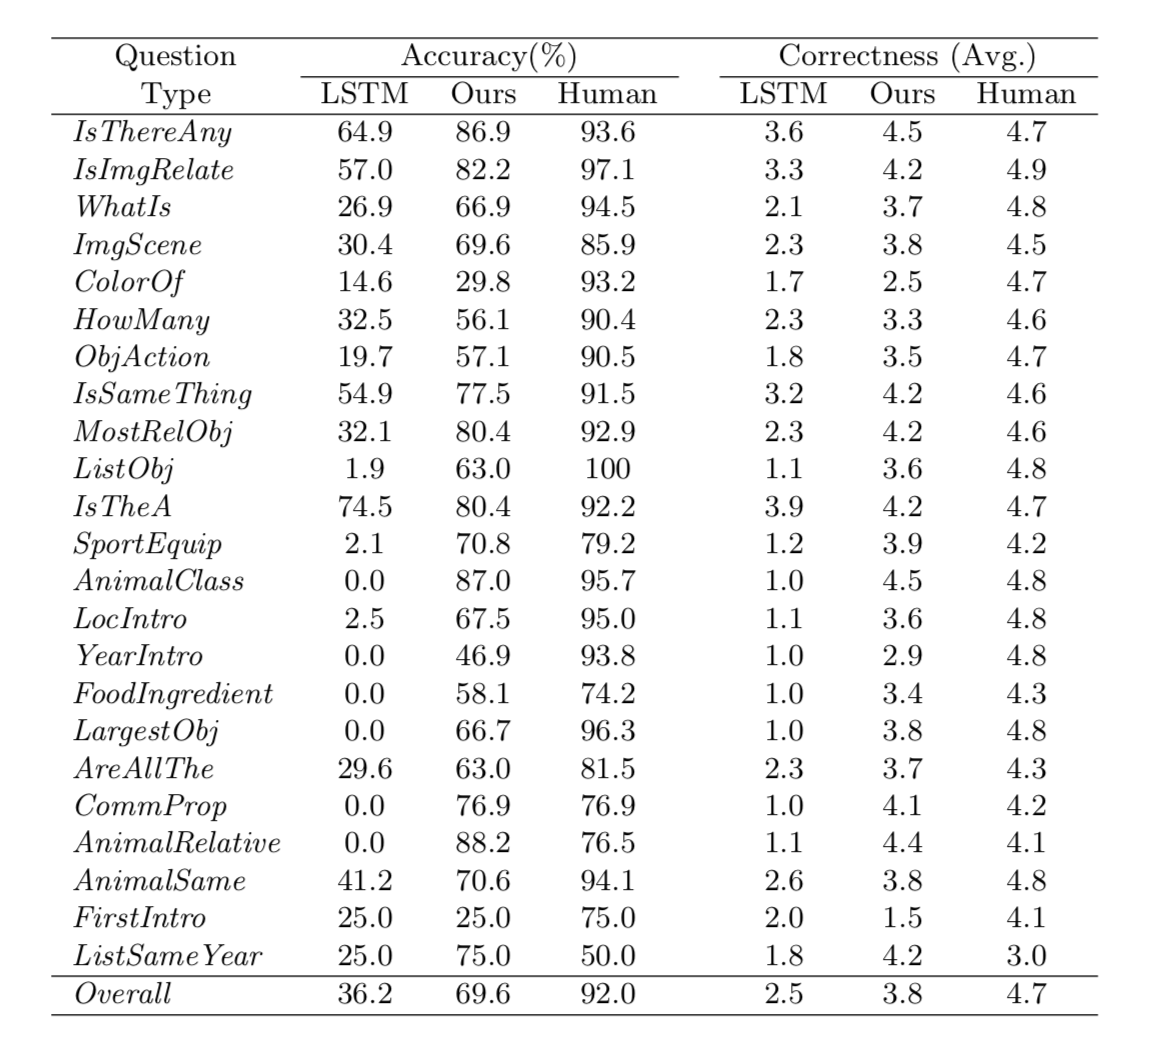
\includegraphics[width=0.8\textwidth]{ahab_evaluation.png}
	\caption{Ahab、联合嵌入模型和人类作答在23种问题上的表现。Accuracy是得分超过3的问题数量的比例,Correctness是某类问题得分的加权平均数。}
	\label{ahab_evaluation}
\end{figure}
KB-VQA将23种问题类型划分为“视觉问题”、“常识问题”、“知识库问题”三个知识等级,如图\ref{qtd},三种不同方法在三种知识等级的正确率统计如图\ref{type_evaluation}。
\begin{figure}[H]
	\centering
	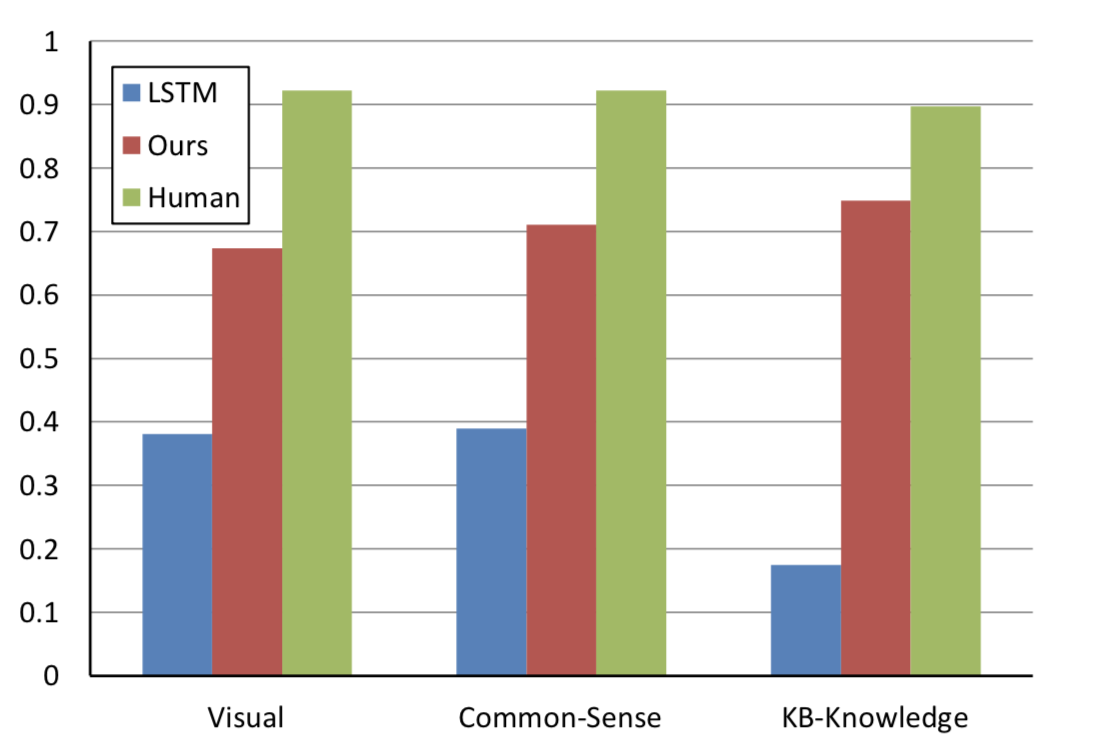
\includegraphics[width=0.8\textwidth]{type_evaluation.png}
	\caption{三种不同方法在三种知识等级的正确率统计}
	\label{type_evaluation}
\end{figure}

从图\ref{qtd}中可以看出,LSTM的联合嵌入模型在“判断动物类别”、“判断对象生产年份”、“列出不同对象的共同属性”、“列出食物营养成分”、“判断最大/最小的物体”、“列出动物的近亲”这六种任务中正确率为0,其中除去“判断最大/最小的物体”为视觉问题外,其余5种问题均需要系统结合额外的知识回答,这正是基于训练集的概率模型的劣势——对于复杂关系和长知识链条的学习能力。总体上看,Ahab在每种问题类型上都优于联合嵌入模型,但离人类的正确率还是有一定差距,尤其在“判断物体颜色”和“比较两个物品的诞生先后”两种问题。

对于“列出与某个物品相同年份的物品”这类问题上,Ahab以75\%的准确率高出人类的50\%,但值得注意的是,KB-VQA数据集中此类问题只有4个,也就是说Ahab只是比人类多答对一个问题,考虑到答案生成过程和正确性评估过程中可能产生的误差,这并不能肯定的表明Ahab系统在此类问题上优于人类的表现。同样的状况也出现在其他问题类型上,因此KB-VQA在不同问题类型上数量的不均衡(问题数最多的类型与问题数最少的类型数量相差两个数量级)和问题样本数过小(16种问题类型的数量小于100,其中有两种的问题数量小于10)在评估视觉问答系统的真实推理能力上不能产生置信度足够高的结果,丰富数据集的样本和均衡不同类型的样本数量才能更好得评估系统的推理表现。

除了测试集存在稳定性较低和样本数较少的问题以外,Ahab系统只能针对预先设定的23种问题类型,这大大限制了问题的开放程度,不能满足真实的问答环境中海量的问题类型。而且Ahab的高正确率还建立在针对性地生成不同的问题查询语句之上,当问题类型数量剧增时,人工的对每种类型设定对应的算法是不切实际的,因此Ahab系统的扩展性也面临挑战。

但相较于主流使用统计方法的联合嵌入模型,Ahab利用知识库取代知识学习过程的方法在复杂推理任务,尤其是需要运用先验知识的问题上,实现了更好的系统表现,也为解决复杂推理问题的方法上提供了有益的实践。

\textbf{FVQA}
Ahab将问题解析为知识库查询语句时,需要预先确定问题模板,这极大的限制了系统面对多样化问题的能力,因此Wang等人改变了问题到查询语句的映射方式提出了FVQA模型\citing{wang2017fvqa}。文章还提出了一个加入fact的数据集,FVQA数据集中的数据格式为(图片,问题,答案,支持事实),支持事实是一个包含答案的资源描述框架(RDF)数据,例如,(猫,能,爬树)。FVQA数据集中的问题包含三个属性:视觉概念(包含物体对象、场景和行为三种类型)、谓语(12种类型)和答案来源(图像和知识库两种)。FVQA模型在训练阶段,从标注后的支持事实中提取出问题的三种属性(VC表示视觉概念类型、REL表示谓语类型、AS表示知识来源类型),由于FVQA数据集中三种属性之间的组合能形成28类问题,所以FVQA模型使用长短期记忆(LSTM)网络训练一个28类的查询语句分类器,实现将问题到查询语句的分类过程,28种查询类型及其在训练/测试集的分布如图\ref{fvqa_query}。
\begin{figure}[H]
	\centering
	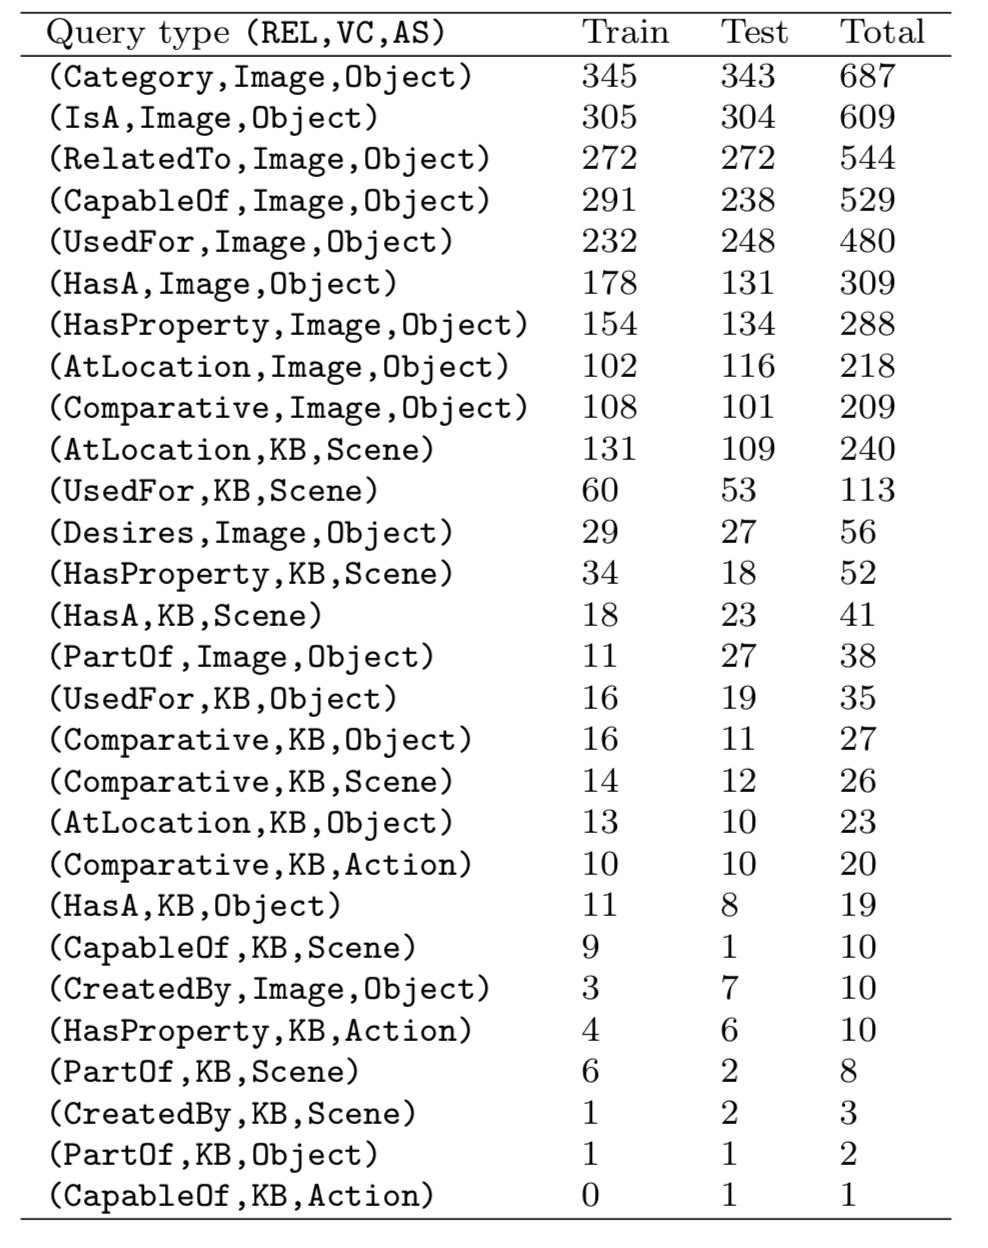
\includegraphics[width=0.5\textwidth]{fvqa_query.png}
	\caption{FVQA模型的28种查询类型及其在训练/测试集的分布情况}
	\label{fvqa_query}
\end{figure}

通过LSTM的分类,文本问题被映射为(REL, AS, VC)的查询类型,对于所有28种查询类型,查询语句都由下面的形式构成:
\begin{verbatim}
Find ?X, ?Y, subject to 
	{(ImgID,Contain,?X) and (?X,VC-Type,VC) and (?X,REL,?Y)}
\end{verbatim}
其中ImgID表示图片的标号,?X表示在图片ImgID中类型为VC的视觉概念,?Y表示在知识库中与?X通过谓语REL链接的概念。再根据AS是图片还是知识库的类型,使用不同的方法得到最终的答案。

FVQA模型中最核心的部分是将问题映射为对应的查询类型,图\ref{qqmaping}展示了问题到查询映射模型(QQmaping)在测试集中对应的三个知识库的正确率,可以看到映射模型在WebChild上实现了超过90\%的高正确率,但在其他两个知识库的准确率就相对较低,分析其中原因,可能是训练集和测试集中问题表达形式相似度的影响。WebChild中的谓语由图\ref{fvqa_vc}可知,都是两者比较的词汇,因此问题的表达形式较为单一,例如,“在图中什么物体更为<形容词的比较级>?”。
\begin{figure}[H]
	\centering
	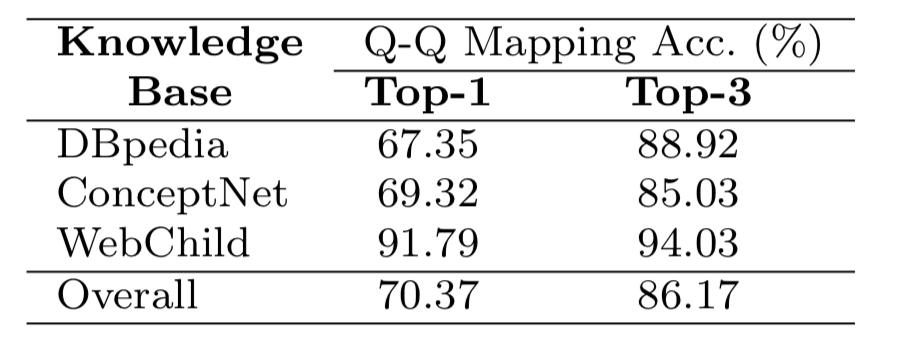
\includegraphics[width=0.5\textwidth]{qqmaping.png}
	\caption{问题到查询映射模型(QQmaping)在测试集中对应的三个知识库的正确率/测试集的分布情况}
	\label{qqmaping}
\end{figure}
引入支持向量机(SVM)\citing{chang2011libsvm}和使用长短期记忆(LSTM)的联合嵌入模型\citing{wu2016value}作为基线模型:只提供问题的SVM-Question和LSTM-Question、只提供图片的SVM-Image和LSTM-Image以及同时提供问题文本和图片的SVM-Question+Image和LSTM-Question+Image,各模型使用FVQA数据集作为训练和测试集中测试,不同模型的正确率见表\ref{fvqa_table}。
% Please add the following required packages to your document preamble:
% \usepackage{multirow}
% \usepackage[table,xcdraw]{xcolor}
% \usepackage{booktabs}
% If you use beamer only pass "xcolor=table" option, i.e. \documentclass[xcolor=table]{beamer}
\begin{table}[H]
% \resizebox{0.5\textwidth}{!}{}
\caption{不同模型在FVQA数据集上的测试正确率,Top-1表示只取得分最高的预测结果,Top-3和Top-10以此类推。灰色数据表示使用与问题对应的完全正确的查询类型时的正确率。}
\begin{tabular}{lccc}
\toprule
\multicolumn{1}{c}{} & \multicolumn{3}{c}{Overall Acc. (\%)}\\
\cmidrule(r){2-4}
\multicolumn{1}{c}{\multirow{-2}{*}{\textbf{Method}}} & \textbf{Top-1}& \textbf{Top-3} & \textbf{Top-10} \\
\midrule
SVM-Qusetion        & 11.19 & 20.68 & 32.14 \\
SVM-Image           & 17.55 & 30.75 & 49.02 \\
SVM-Qusetion+Image  & 17.99 & 31.83 & 49.55 \\
LSTM-Question       & 10.30 & 18.26 & 31.02 \\
LSTM-Image          & 22.69 & 36.21 & 58.59 \\
LSTM-Question+Image & 23.37 & 37.02 & 52.51 \\
\midrule
\cellcolor[HTML]{C0C0C0}gt-QQmaping & \cellcolor[HTML]{C0C0C0}64.23 & \cellcolor[HTML]{C0C0C0}71.58 & \cellcolor[HTML]{C0C0C0}72.74 \\
top-1-gt-QQmaping & 53.63 & 60.70 & 61.59 \\ 
top-3-gt-QQmaping & \textbf{58.19} & \textbf{65.89} & \textbf{66.83} \\
\bottomrule
\end{tabular}
\label{fvqa_table} 
\end{table}

从表\ref{fvqa_table}中Top-1一列可以看出,无论是SVM-Question+Image与SVM-Image之间的正确率差距还是LSTM-Question+Image与LSTM-Image的正确率差值都非常小,这说明问题的解析对于SVM和LSTM这两种模型正确率的提升没有太大的帮助,而两个模型总体的正确率也处于较低的水平,说明统计方法在样本较小的语料库中很难学习到知识间真正的逻辑关联。而FVQA模型使用问题到查询映射模型能从问题文本中提取到关键信息,并能利用关键信息组成有意义的语言结构,再结合额外知识库搜索到正确答案,答案获得的过程反映了推理的过程。gt-QQmaping(灰色背景)使用问题对应的正确查询类型,因此正确率反映了理想状况下FVQA模型从查询类型到生成查询语句过程中的误差情况,知识库查询过程的错误率在30\%左右。top-1-gt-QQmaping与gt-QQmaping之间的差距则代表问题到查询类型70.37\%(见图\ref{qqmaping})的正确率在最终答案的影响,top-3-gt-QQmaping的准确率高于top-1-gt-QQmaping的原因在是因为前者拥有更高的问题到查询类型映射的准确率。

表\ref{fvqa_answerSource}提供了不同方法在不同答案来源上的正确率,对比表中Image和KB两列容易看出,答案来源于视觉概念的准确率在所有模型上均远高于知识库来源,这说明表中涉及的三种模型都只能从图像和问题文本中包含的概念中提取答案,一旦答案涉及都额外知识库中的“新”概念,准确率便急剧下降,即使是使用额外知识库的gt-QQmaping。
\begin{table}[H]
% \resizebox{0.8\textwidth}{!}{}
\centering
\caption{不同方法在不同答案来源上的正确率}
\begin{tabular}{lcccccc}
\toprule
\multicolumn{1}{c}{\multirow{3}{*}{\textbf{Method}}} & \multicolumn{6}{c}{Answer-Source}\\
\cmidrule(r){2-7}
 & \multicolumn{3}{c}{\textbf{Image}} & \multicolumn{3}{c}{\textbf{KB}}\\
\cmidrule(r){2-4}
\cmidrule(r){5-7}
 & \textbf{Top-1} & \textbf{Top-3} & \textbf{Top-10} & \textbf{Top-1} & \textbf{Top-3} & \textbf{Top-10} \\
 \midrule
SVM-Qusetion        & 12.80 & 24.53 & 36.48 & 0.68 & 2.03 & 3.72 \\
SVM-Image           & 19.92 & 34.88 & 55.11 & 2.03 & 3.72 & 9.12 \\
SVM-Qusetion+Image  & 20.43 & 36.07 & 55.73 & 2.03 & 4.05 & 9.12 \\
LSTM-Question       & 11.71 & 20.49 & 34.21 & 1.01 & 3.72 & 10.14 \\
LSTM-Image          & 25.49 & 40.40 & 65.12 & 4.39 & 8.78 & 15.88 \\
LSTM-Question+Image & 26.01 & 41.12 & 58.05 & 6.08 & 10.14 & 16.22 \\
\midrule
\cellcolor[HTML]{C0C0C0}gt-QQmaping & \cellcolor[HTML]{C0C0C0}72.65 & \cellcolor[HTML]{C0C0C0}80.13 & \cellcolor[HTML]{C0C0C0}80.13  & \cellcolor[HTML]{C0C0C0}9.12 & \cellcolor[HTML]{C0C0C0}15.54 & \cellcolor[HTML]{C0C0C0}24.32 \\
top-1-gt-QQmaping & 60.89 & 68.27 & 68.27 & 6.08 & 11.15 & 17.91 \\ 
top-3-gt-QQmaping & \textbf{66.10} & \textbf{74.15} & \textbf{74.15} & \textbf{6.42} & \textbf{11.82} & \textbf{18.92} \\
\bottomrule
\end{tabular}
\label{fvqa_answerSource}
\end{table}

FVQA模型提出了一种以句法结构中的谓语为核心的先验知识问题的解答思路,首先从问题中解析出关键的谓语信息,在问题到查询类型模型中,结合谓语、视觉概念和答案来源决定了28种不同的查询类型,再使用生成的查询语句搜索基于12种谓语构建的知识库,最终预测答案。“主语-谓语-宾语”的一般句式结构中谓语表示了主语和宾语之间的相互作用,即使在相同的主语和宾语情况下,不同的谓语能表达出截然不同的语义信息,而绝大多数问题也能够直接通过谓语,推断答案的范畴。以谓语为基础的优势有几点,第一,易于问题分类。问题的自然语言表达方式众多,但无论如何改变句式结构,表达相同含义的谓语有限,通过对谓语的语义划分能够划分出问题的不同类型。第二,便于知识库的查询。知识库中的实体之间通过不同的谓语连接,形成错综复杂的知识网络,一个实体有众多连接,但一个谓语只连接两个实体,且往往谓语的两端就是问题的答案。

FVQA模型的缺陷有三点,第一,分类数量的确定和分类模型的精度。FVQA模型由于查询语句的生成依赖于查询类型,因此问题到查询类型映射的准确性会直接影响到答案生成的正确率。表\ref{fvqa_table}是在FVQA数据集上进行的,由于数据集中问题的类型只有28种,因此FVQA模型在问题到查询类型映射模型中使用了28类的分类器,但在实际问答环境中问题类型的具体数量远远多于28种,且无法预先确定。想训练能应用于实际情景中,FVQA模型不仅需要数据集的扩充,还需要提高模型本身的分类精度。第二,不能回答以谓语为答案的问题。所有28种查询类型都要求能从问题中提取关键谓语,并且所有答案都是物体对象,如果问题询问对象之间的关系,模型则无法从问题文本中获得谓语,不能得到答案。第三,不能很好的处理含有多个动词的复杂推理问题。FVQA模型的查询语句过于简单,仅仅将一次查询结果作为答案,在面对需要多级推理的问题时,便无法直接得到答案,如表\ref{fvqa_wrong}。
\begin{table}[H]
% \resizebox{0.8\textwidth}{!}{}
\centering
\begin{tabular}{lcccccc}
\toprule
\multicolumn{2}{c}{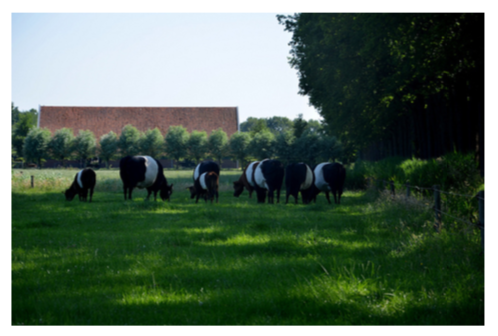
\includegraphics{cow.png}} \\
\multicolumn{2}{c}{What is related to the animal that can be found in this place?} \\
\midrule
\multirow{2}{*}{Mined Facet:} & You are likely to find a cow in a picture \\
 & The cow is related to the tree \\
Predicted Answer: & cow \\
Ground Truth: & tree \\
\bottomrule
\end{tabular}
\caption{问题中包含related和found两个动词,FVQA模型只能提取一个作为谓语并查询,选择found为谓语时,会出现错误的预测}
\label{fvqa_wrong}
\end{table}

\textbf{基于知识库的通用嵌入模型}
无论是Ahab还是FVQA模型都是通过将问题固定在一定类型,再通过对应不同问题的类型的额外知识库查询,获得更丰富的知识,从而提高复杂问题的正确率。为了提高视觉问答系统的问题的灵活性,Wu等人又通过改进常见的CNN+LSTM的嵌入模型,提出了基于知识库的通用嵌入模型。模型的基本架构由图像属性提取网络(CNN)、图像描述生成网络、外部知识库查询网络以及答案生成网络(LSTM)构成,模型架构如图\ref{KBLSTM}。
\begin{figure}[H]
	\centering
	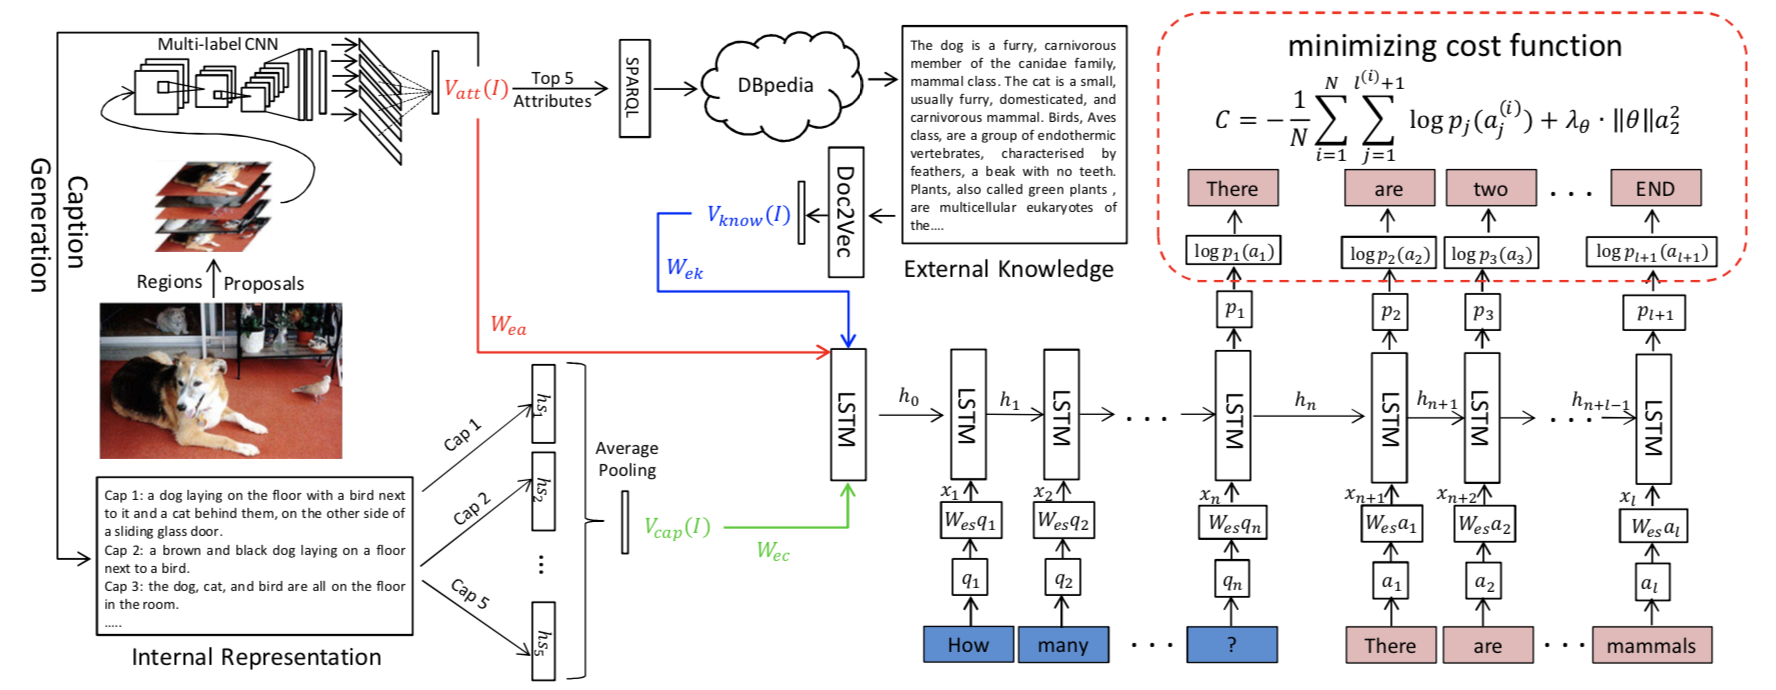
\includegraphics[width=0.8\textwidth]{KBLSTM.png}
	\caption{结合外部知识库的通用嵌入模型}
	\label{KBLSTM}
\end{figure}

图像属性提取网络将图像属性提取问题视为多标签的分类问题,以图像的多个子区域作为输入,输出前五个从MS COCO中筛选得到的图像属性$V_{att}(I)$,属性可能为物体名称、动作或者描述特征的形容词。提取出的图像属性分别作为图像描述生成网络和外部知识库查询网络的输入,图像描述生成网络将\cite{wu2016value}中的高层次的属性表达输入LSTM网络生成基于图像属性的描述,再将文本描述转化为五个特征向量,平均池化所有向量得到向量$V_{cap}(I)$。外部知识库查询网络首先分别将五个图像属性转化为知识库查询语言,查询到DBpedia知识库中相应的对象后,返回其“comment”——“comment”往往包含关于知识库对象最重要的解释信息,如图\ref{SPAQLexample},为了将大段的“comment”转化为向量,Wu等人使用Doc2Vec\citing{le2014distributed}——一种能方便的将句子、段落甚至文章等不固定长度的文本转化为固定大小的向量的模型,并且能包含文本内容的语义信息。——将其转化为$V_{know}(I)$。最后将$V_{att}(I)$、$V_{cap}(I)$、$V_{know}(I)$以及问题文本作为答案生成网络(LSTM)的输入,训练网络生成答案。
\begin{figure}[H]
	\centering
	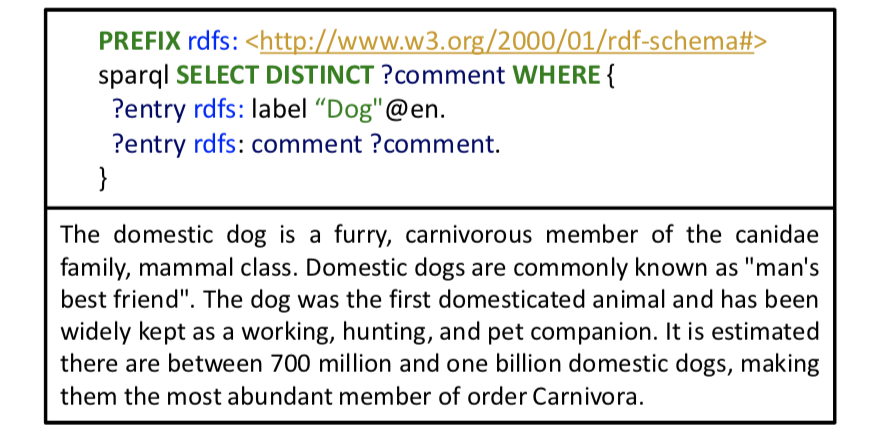
\includegraphics[width=0.5\textwidth]{SPAQLexample.png}
	\caption{使用‘dog’属性的查询语句以及返回的‘comment’内容}
	\label{SPAQLexample}
\end{figure}

在评估模型准确率时,由于该模型面对开放性问题,因此不同于Ahab和FVQA只能使用专门设计的数据集,该模型采用Toronto COCO-QA\citing{ren2015exploring}和VQA\citing{antol2015vqa}两个数据集进行评测。为了说明该模型的正确率情况,引入基线模型和几个结果较优的模型正确率作为对比,GUESS表示随机猜测模型,VggNet-LSTM使用在ImageNet上预处理的VggNet网络连接LSTM得到,VggNet+ft-LSTM使用在图像属性分类任务上微调后的VggNet,Att-LSTM表示直接将$V_{att}$作为LSTM输入的变体模型,类似的变体有Att+Cap-LSTM、Att+Know-LSTM、Att+Cap-LSTM、Cap+Know-LSTM,以及完整的Att+Cap+Know-LSTM模型。不同模型在两个数据集的正确率分别如表\ref{Wucoco}和\ref{Wuvqa}。
\begin{table}[H]
% \resizebox{0.8\textwidth}{!}{}
\centering
\caption{不同模型在Toronto COCO-QA正确率的表现}
\begin{tabular*}{0.6\textwidth}{@{\extracolsep{\fill}}lc}
\toprule
\textbf{Toronto COCO-QA} & Acc(\%)\\
\midrule
GUESS\citing{ren2015image} & 6.65 \\
VggNet-LSTM & 50.73 \\
VggNet+ft-LSTM & 58.34 \\
\midrule
Att-LSTM & 61.38 \\
Att+Cap-LSTM & 69.02 \\
Att+Know-LSTM & 63.07 \\
Cap+Know-LSTM & 64.31 \\
\midrule
Att+Cap+Know-LS & \textbf{69.73} \\
\bottomrule
\end{tabular*}
\label{Wucoco}
\end{table}

\begin{table}[H]
% \resizebox{0.8\textwidth}{!}{}
\centering
\caption{不同模型在VQA数据集的正确率表现}
\begin{tabular*}{0.6\textwidth}{@{\extracolsep{\fill}}lc}
\toprule
\textbf{VQA} & Acc(\%)\\
\midrule
VggNet-LSTM & 44.93 \\
\midrule
Att-LSTM & 51.60 \\
Att+Cap-LSTM & 55.04 \\
Att+Know-LSTM & 53.79 \\
Cap+Know-LSTM & 52.31 \\
\midrule
Att+Cap+Know-LS & \textbf{55.96} \\
\bottomrule
\end{tabular*}
\label{Wuvqa}
\end{table}

虽然该模型名义上是使用了外源知识库,但实际上其还是沿袭了联合嵌入模型的思路,并没有使用知识库中的结构化内容,而是在图像特征和文本特征中加入了额外的文本特征。也正是因为这种改动,使得其能使用更通用的数据集进行模型评估,但实际效果一般。

总结上文提到的所有视觉问答模型,可以看出联合嵌入模型是主流,注意力机制和动态记忆网络的出现也都是为了弥补原有联合陷入模型的计算效率不高、记忆短缺等问题。虽然引入外源知识库能更为彻底的解决神经网络知识存储不足的问题,实现特征提取和答案推理的分离,但是值得注意的是,如果希望使用知识库的结构化知识提高模型的解释性和作答更复杂的推理问题,如何实现高效率的答案搜索成为关键。一方面,人工设计的问题类型能极大的规范搜索方式,为进一步优化搜索算法提供基础,但另一方面,因为自然语言的多样性和变化性,问题类型的人工设计成本会随之提高,并且对于监督学习而言,数据集的标注也成为了成本骤增的重要负担,这也是为什么使用知识库的模型需要额外设计数据集的原因。如何在提高知识库搜索算法的准确性的同时,保证数据集的开放性这是一个值得深入研究的问题,文本将针对这个问题做出一些具有价值的尝试和开拓。

\section{本文的主要贡献与创新}
正如以上提到的诸多模型的探索,视觉问答领域正在迎来百花齐放的局面。模型的多样性和答案的准确率会同时受惠于目前机器学习在计算机视觉、自然语言处理和知识表达与推理的成功应用。然而,除了颇具前景的应用方向和深远的研究意义,视觉问答仍然属于起步阶段,面临着诸多亟待解决的问题。我们认为现有的模型还存在以下三个主要问题。

第一,泛化能力受限于数据集。目前的视觉问答主流模型为联合嵌入模型,其主要思路为联合图像处理模型输出的图像特征和自然语言处理输出的文本特征,并利用神经网络训练联合后的特征,得到答案。和其他基于神经网络的模型一样,联合嵌入模型的泛化性能主要由训练集的大小、内容的多样性等因素影响。然而数据集的收集和整理工作需要消耗大量的的人工成本,因此“数据集偏见”成为目前模型泛化性能的主要瓶颈之一。

第二,结果的可解释性匮乏。目前的视觉问答模型大多仍然属于分类模型,候选答案来源于训练集,模型对候选答案评分,并将得分最高的候选答案作为输出。而分类的标准存在于模型中的大量参数之中,模型得出答案的过程和标准并不明确。匮乏的可解释性在需要多步推理的问题上表现尤为突出。该类问题不同于识别任务,答案的得出是分步进行的,每一步的正确推理都对答案的得出至关重要。而通过分类模型得出的答案无法给出每一步的推理过程。

第三,缺少通用架构。正如以上提到的,联合嵌入模型和基于知识库的视觉问答模型是目前研究的重点方向。基于知识库的视觉问答模型的提出是为了解决训练集的有限性和答案的黑盒性。外源知识库能够扩展模型可搜寻的答案范围,结构化且语义明确的实体之间的关系也可以提供答案的可解释性。然而,目前基于知识库的视觉问答模型根据各自的特点建立独特的数据集,该类自建的数据集从数据量和多样性的角度都不如通用的数据集,例如VQA2.0\citing{goyal2017making}。因此由于使用的数据集不同,目前两个主要的研究方向的模型之间很难建立统一的标准以衡量性能之间的差异性,造成了联合嵌入模型和基于知识库的VQA模型的割裂。

为解决第一个问题中提到的数据集限制,我们依照答案和源信息相关性,研究了主要的视觉问答数据集,并且从中选择数据集构成实验数据集。实验数据集需要包含QI、Qi、qI、qi全部四种问题类型,从而扩展问题类型的多样性。至于数据集的数据量扩展并不在本文的研究范围之内。

为了实现联合嵌入模型和基于知识库的VQA模型的融合,我们试图构建一个能处理四种问题类型统一架构,因此提出了一个通用的视觉问答架构——KB-Specific Network(KBSN)模型。本文的主要贡献和创新点如下:

1. 对于视觉问答问题,我们根据答案分别与问题和图像之间的依赖性的不同,提出了一个视觉问答类型的划分标准,划分出QI、Qi、qI、qi四种问题类型。并使用该标准解释了联合嵌入模型与基于知识库的模型的差异。

2. 构建了一个联合嵌入模型——None KB-Specific Network(N-KBSN)模型。N-KBSN模型由
三个主要部分组成:问题文本和图像特征提取模块、自注意力和引导注意力模块、 特征融合和分类器。其中,图像特征提取器为 Faster R-CNN \citing{ren2015faster},问题文本特征提取使用 ELMo 模型 \citing{Peters:2018},并使用从 Transformer 中借鉴的多头注意力机制分别实现图片的自注意力(V-SA)、 问题文本的自注意力(Q-SA)、由问题引导的对图像的注意力(Guided Attention, GA),最后通过特征融合预测答案。

3. 区别于其他基于知识库的视觉问答模型,我们提出将知识库转化为图嵌入——使用低维特征向量表示与问题相关的知识子图,而不是使用查询语言获取知识库中的子节点\citing{wang2015explicit, wang2017fvqa}。知识库的图嵌入由子图提取模块和子图嵌入模块两个主要部分组成。子图提取模块的作用是完成从图像和问题文本到知识库的映射。子图嵌入模块是将提取得到的子图映射为图嵌入。知识库的图嵌入能表达实体之间的结构信息,从而增强特征的表达能力。并且低维的特征向量具有计算便利性,可以实现大规模的训练和预测,消除了人工设计查询语言的复杂性。

4. 在N-KBSN模型的基础上,融合知识库的图嵌入,提出一个通用的视觉问答架构——KB-Specific Network(KBSN)模型。KBSN 模型使用了 N-KBSN 模 型的问题文本和图像特征提取模块、自注意力和引导注意力模块,而在特征融合 时引入了知识库的图嵌入。

\section{本论文的结构安排}
本文的章节结构安排如下:

第一章,绪论。本章节主要介绍了视觉问答任务的研究内容和应用前景,提出了一种新的问题类型的划分标准,还对视觉问答的国内外研究状况作了比较完整的归纳,其中重点介绍了已有的联合嵌入模型和基于知识库的模型,最后阐述和总结本文的研究内容。

第二章,视觉问答数据集。本章对已有的主要的视觉问答数据集进行了概括性的介绍,并且根据数据集的问题是否需要外源知识为标准,分为基于视觉的数据集和基于知识的数据集,最后介绍了本文使用的实验数据集及其选取策略。

第三章,None KB-Specific Network(N-KBSN)。本章首先分析了联合嵌入模型在视觉问答任务优异表现的原因,并据此提出了N-KBSN模型,随后详细介绍了N-KBSN模型的问题文本和图像特征提取模块、自注意力和引导注意力模块。其中,使用Faster R-CNN\citing{ren2015faster}提取图像特征,ELMo模型\citing{Peters:2018}提取问题文本特征,使用多头注意力机制\citing{NIPS2017_7181}实现图像的自注意力(V-SA)、 问题文本的自注意力(Q-SA)、由问题引导的对图像的注意力(Guided Attention, GA)。最后使用VQA2.0数据集\citing{goyal2017making}训练和测试模型,并且通过剔除实验分析了各个模块在模型中的作用,通过和其他最优模型的比较证明了其有效性。

第四章,KB-Specific Network(KBSN)。本章简要介绍了知识库的发展历史,并且分析了几个重要的知识库各自的特点。随后提出了使用图嵌入的模式表示知识库,并在上一章提出的N-KBSN模型的基础上,提出了一个通用的视觉问答架构——KB-Specific Network(KBSN)模型,最后使用KB-VQA\citing{wang2015explicit}和FVQA\citing{wang2017fvqa}数据集训练和测试模型,通过对比其他模型,分析实验结果,证明了KBSN模型在回答常识型问题和知识型问题的优越性。

第五章,全文总结与展望。主要总结全文研究内容及结论,并阐述后续工作的主要研究方向。

